
\documentclass[11pt]{report} %Type de doc. %scrartcl   scrreprt

% TEMPORARY
\usepackage{soul}


% standard
\usepackage[french,english]{babel}
\usepackage[utf8]{inputenc} %Caracteres accentués           
\usepackage[T1]{fontenc} 	%Police accentuée
\usepackage{lmodern}			%Police vectorielle (haute qualité)
\usepackage{vmargin} %Marges normales en A4
\usepackage{amsmath} %Insertion d'equations
\usepackage{todonotes}


\usepackage{amssymb}
\usepackage{vmargin} 

\usepackage{graphicx} %Images dans le PDF
\usepackage{float} 		%Flottants : Figures,Tables
\usepackage{color}		%Utilisation de couleurs
\definecolor{gris}{gray}{0.5}
\usepackage{eurosym}
\usepackage[hyphens]{url}
\usepackage{hyperref}
% \usepackage{breakurl}
\usepackage{wrapfig}
\usepackage{multirow} 
\usepackage{rotating}
\usepackage[small,bf]{caption}
\usepackage{textcomp}
\usepackage{slashbox}
\usepackage{subfig} 

\usepackage{amsthm}
\usepackage{pgf}

\usepackage{epstopdf}
\usepackage{attachfile} 
\usepackage{longtable}

\usepackage[framemethod=tikz]{mdframed}

\theoremstyle{plain}
\newtheorem{example}{{\bf Example}}[chapter]
\numberwithin{example}{chapter}
\newtheorem{theorem}{{\bf Theorem}}[chapter]
\numberwithin{theorem}{chapter}
\newtheorem{proposition}{{\bf Proposition}}[chapter]
\numberwithin{proposition}{chapter}
% \newtheorem{property}[example]{{\bf Property}}
\newtheorem{definition}{{\bf Definition}}[chapter]
\numberwithin{definition}{chapter}
\newtheorem{lemma}{{\bf Lemma}}[chapter]
\numberwithin{lemma}{chapter}
\newtheorem{property}{{\bf Property}}[chapter]
\numberwithin{property}{chapter}
% \newtheorem{hypothesis}[example]{{\bf Hypothesis}}
% \newtheorem{exercise}{{\bf Exercise}}[section]
\newtheorem{thesis}{Thesis}[chapter]
\numberwithin{thesis}{chapter}
\theoremstyle{remark}
\newtheorem*{remark}{Remark}%[chapter]
% \numberwithin{remark}{chapter}

\surroundwithmdframed[outerlinewidth=2,roundcorner=10pt,leftmargin=0,rightmargin=0,% backgroundcolor=yellow!40,outerlinecolor=blue!70!black,
innertopmargin=\topskip,splittopskip=\topskip,ntheorem=true, nobreak=true]{theorem}
\surroundwithmdframed[outerlinewidth=2,roundcorner=10pt,leftmargin=0,rightmargin=0,% backgroundcolor=yellow!40,outerlinecolor=blue!70!black,
innertopmargin=\topskip,splittopskip=\topskip,ntheorem=true, nobreak=true]{lemma}
\surroundwithmdframed[outerlinewidth=2,roundcorner=10pt,leftmargin=0,rightmargin=0,% backgroundcolor=yellow!40,outerlinecolor=blue!70!black,
innertopmargin=\topskip,splittopskip=\topskip,ntheorem=true, nobreak=true]{thesis}
 

\setcounter{secnumdepth}{3}
\setcounter{tocdepth}{3}

\newcommand{\E}{\mathbb{E}}
\newcommand{\R}{\mathbb{R}}

\allowdisplaybreaks[3] % ou x prend une valeur entière comprise entre 0 et 4; Plus x est gd, plus le compilateur accepte les coupures sur deux pages dans une formule.
% permet que les align puissent se prolonger sur pls pages

%========================================
\usepackage{listings}	%Inclusion de code-source
\lstset{							%Paramètres généraux pour les inclusions de code
	  language=matlab,
    basicstyle=\ttfamily\small,
    aboveskip={1.0\baselineskip},
    belowskip={1.0\baselineskip},
    columns=fixed,
    extendedchars=true,
    breaklines=true,
    tabsize=4,
    prebreak=\raisebox{0ex}[0ex][0ex]{\ensuremath{\hookleftarrow}},
    frame=lines,
    showtabs=false,
    showspaces=false,
    showstringspaces=false,
    keywordstyle=\color[rgb]{0.627,0.126,0.941},
    commentstyle=\color[rgb]{0.133,0.545,0.133},
    stringstyle=\color[rgb]{01,0,0},
    numbers=left,
    numberstyle=\small,
    stepnumber=1,
    numbersep=10pt,
    captionpos=t,
    escapeinside={\%*}{*)}
	}
\renewcommand{\lstlistingname}{\textsc{Algorithm}}	%Remplacer 'Listing' par 'Code' dans les légendes
%\usepackage[french,boxed,linesnumbered]{algorithm2e}	%Package algorithme avec options
\usepackage[english,algoruled, linesnumbered]{algorithm2e}	%Package algorithme avec options

\hypersetup{
colorlinks,%
citecolor=black,%
filecolor=black,%
linkcolor=black,%
urlcolor=black
} 

\makeatletter
\def\url@leostyle{%
  \@ifundefined{selectfont}{\def\UrlFont{\sf}}{\def\UrlFont{\small\ttfamily}}}
\makeatother
%% Now actually use the newly defined style.
\urlstyle{leo}


 \usepackage{layout}
% \usepackage{geometry}
 \usepackage{array}
 \usepackage{fancyvrb}
 \usepackage[parfill]{parskip} % espace apres paragraph
%% \usepackage{fourier} % not to use
\usepackage{pdfpages}
%
\newcommand{\QED}{\begin{flushright} QED \end{flushright}}
\newcommand{\ent}[1]{\lfloor #1 \rfloor}
\newcommand{\ceil}[1]{\lceil #1 \rceil}
\newcommand{\tup}[2]{\left( \begin{matrix} #1\\ #2\end{matrix} \right)}

% section numbering type
\renewcommand\thechapter{\Alph{chapter}}
\renewcommand\thesection{\arabic{section}.}
\renewcommand\thesubsection{\alph{subsection}.}
\renewcommand\thesubsubsection{\roman{subsubsection}.}

\usepackage{titlesec}
\titlespacing*{\subsection}
  {15pt}% decalage a gauche (positif ou negatif)
  {3.5ex plus 1ex minus .2ex}% espacement vertical avant
  {2.3ex plus .2ex}% espacement vertical apres
\titlespacing*{\subsubsection}
  {30pt}% decalage a gauche (positif ou negatif)
  {3.5ex plus 1ex minus .2ex}% espacement vertical avant
  {2.3ex plus .2ex}% espacement vertical apres

\usepackage{framed}

\renewenvironment{proof}{{\bfseries Proof}}{\QED}

\usepackage{tocstyle}
\usetocstyle{standard}

\usepackage{tikz}
\usetikzlibrary{shapes,arrows,calc,decorations.pathmorphing,decorations.pathreplacing}
\tikzset{snake arrow/.style=
{->,
decorate,
decoration={snake,amplitude=.4mm,segment length=2mm,post length=1mm}},
}

\usepackage{array}
\newcolumntype{L}[1]{>{\raggedright\let\newline\\\arraybackslash\hspace{0pt}}m{#1}}
\newcolumntype{C}[1]{>{\centering\let\newline\\\arraybackslash\hspace{0pt}}m{#1}}
\newcolumntype{R}[1]{>{\raggedleft\let\newline\\\arraybackslash\hspace{0pt}}m{#1}}

% shortcuts
\newcommand{\vnorm}[1]{\left\Vert #1 \right\Vert}
\newcommand{\myspan}{\mathrm{span}} % span
\newcommand{\myint}{\mathrm{int}} % span
\newcommand{\e}{\mathrm{e}} % e for exponential
\newcommand{\dd}{\mathrm{d}} % d differential
\newcommand{\J}{\mathrm{J}} % jacobian
%%%%%%%%%%%%%%%%%%%%%%%%%%%%%%%%%%%%%%%%%%%%%%%%%%%%%%%%%%%%%
%% DOCUMENT
%%%%%%%%%%%%%%%%%%%%%%%%%%%%%%%%%%%%%%%%%%%%%%%%%%%%%%%%%%%%%

\begin{document}

%% page de garde
\newcommand{\HRule}{\rule{\linewidth}{0.5mm}}

\begin{titlepage}
	
\begin{center}

% Upper part of the page

\includegraphics[width=0.30\textwidth]{images/epl.jpg}\\[1cm]    

\textsc{\LARGE Universit\'e catholique de Louvain}\\[1.5cm]

\HRule \\[0.5cm]

\textsc{\Large \bsc{LINMA2471}}\\[0.2cm]
\textsc{\Large Optimization models and methods II}\\[0.5cm]


% Title
\HRule \\[2cm]
{\huge \bfseries Course notes}\\[1cm]

\HRule \\[1.5cm]

% Author
\begin{minipage}{0.8\textwidth}
% \begin{flushleft} 
\large
\emph{Students:}\\
Ismail \bsc{Ad'Oul}, Noé \bsc{Antoine}, Antoine \bsc{Aspeel}, Nicolas \bsc{Boutet}, Sibo \bsc{Cheng}, Benjamin \bsc{Chiem}, Geoffrey \bsc{Ciamarra}, Antoine \bsc{de Comité}, Alexandre \bsc{de Touzalin}, Boris \bsc{Dehem}, François \bsc{Delcourt}, Renaud \bsc{Dufays}, Antoine \bsc{Durviaux}, Céline \bsc{Gérard}, Andine \bsc{Havelange}, Florimond \bsc{Houssiau}, Sébastien \bsc{Lagae}, Quynh \bsc{Le}, Adissa \bsc{Laurent}, Bruno \bsc{Losseau}, Joachim \bsc{Lucas}, Laura \bsc{Motte}, Pierre-Paul \bsc{Mouchet}, Guillaume \bsc{Olikier}, Caroline \bsc{Sautelet}, Vincent \bsc{Schellekens}  \& Leïla \bsc{Van Keirsbilck}
% \end{flushleft}
\end{minipage}







\vfill

% Bottom of the page
{\large  2015}

\end{center}	
	
	
\end{titlepage}


\selectlanguage{english}

\pagenumbering{roman}
\tableofcontents
\newpage
\pagenumbering{arabic}

\part{Notes}

\chapter{Linear and Convex modeling}	
\label{Ch1}
	
%\documentclass[a4paper]{article}
%\usepackage[utf8]{inputenc}
%\usepackage{amsthm}             % Definitions and such
%\usepackage{amssymb}            % R for space and such
%\usepackage{amsmath}
%\usepackage[a4paper]{geometry}
%
%\title{LINMA2471 : Optimization models and models : course 2 (23/09/2015)}
%\author{Antoine de Comité , Florimond Houssiau \& Vincent Schellekens}
%\date{September 2015}
%
%\usepackage{natbib}
%\usepackage{graphicx}
%\usepackage{framed}
%\usepackage{tikz}
%\usepackage{float}
%\usetikzlibrary{arrows}
%\usetikzlibrary{decorations.markings}
%
%
%\begin{document}
%
%
%
%\maketitle

In this chapter we will see some important classes of optimization problems, and some techniques to re-write an optimization problem into another form.

\section{Definitions and motivation}
First of all, let's recall what the model of an optimization problem looks like.\\

\begin{definition}
A \textbf{general model} has the following form :
\begin{equation}
\min_{x \in X \subseteq \mathbb{R}^n} f(x)
\end{equation}
where $x$ are the \textbf{variables}, X is the \textbf{feasible set} (also called domain or feasible region) and f is the \textbf{objective function}.
\end{definition}

Note that the feasible set $X$ is a subset of a \textit{finite} dimensional space. Optimization within infinite-dimensional spaces are not covered in this course.\\

Let us next introduce two very important classes of models : the \textit{linear} and \textit{convex} models.\\

\begin{definition}
A model is called a \textbf{linear model} if :
\begin{enumerate}
  \item The objective function is linear/affine\footnote{Note that the independent term of an affine function ($d$) can be easily dropped out, because it doesn't affect the optimal solution in any way. Therefore, every affine function can be replaced with a purely linear one.}, that is, of the form $c^T x/c^T x +d$.
  \item The feasible set X is a \textbf{polyhedron}. A polyhedron is an intersection of a finite\footnote{For example, a sphere is therefore \textit{not} a polyhedron, because it is an intersection of an \textit{infinite} number of closed half-planes.} number of closed \textbf{half-spaces}. As a reminder, a half-space is the set of points that lie on one side of a hyperplane; in an algebraïc form : $\{x \in \mathbb{R}^n | a^T x \geq b\}$ or $\{x \in \mathbb{R}^n | a^T x \leq b\}$.
\end{enumerate}
\end{definition}

\vspace{\baselineskip}
		
\begin{definition}
A model is called a \textbf{convex model} if :
\begin{enumerate}
  \item The objective function f is convex (see below). 
  \item The feasible set X is convex (see below).
\end{enumerate}
\end{definition}

We still need to define what are convex functions and sets :\\

\begin{definition}
    A set X is a \textbf{convex set} if it contains the segments between every pair of its points.
\end{definition}

\vspace{\baselineskip}

\begin{definition}
    A function f is a \textbf{convex function} if its \textbf{epigraph} is convex. The epigraph\footnote{Note that if $f : \mathbb{R}^n \to \mathbb{R}$ then $epi \: f \subseteq \mathbb{R}^{n+1}$} of f is the set of points above (and including) the graph of f. Formally, we write this as : $epi \: f := \{(x,t)|t \geq f(x)\} $. This notion is illustrated on Figure \ref{epi}.
\end{definition}

For the definition of convex functions, we didn't used the concept of derivative, because we want our definition to be as general as possible. In other words, a non-differentiable function can be convex\footnote{For example, the norm function defined by $f:\mathbb{R} \to \mathbb{R}: x \to |x|$ is convex}. Note also that \textit{every linear model is a particular case of a convex model}.\\


\begin{figure}[h!]
\centering
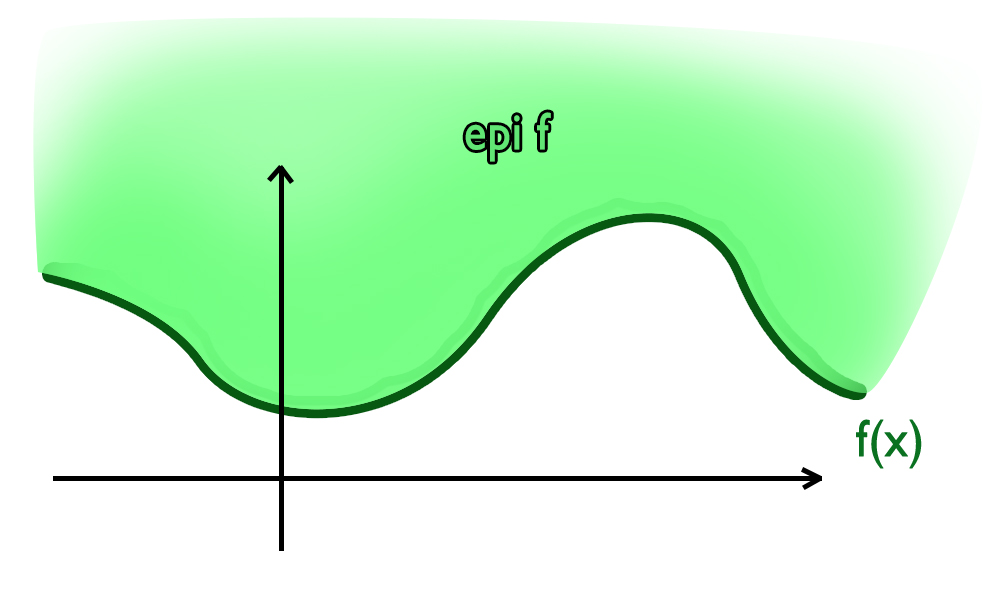
\includegraphics[scale=0.3]{./images/Course2_epi}
\caption{Illustration of the epigraph of some one-dimensional (and non-convex) function. The epigraph of $f$ is the region above the graph of $f$. }
\label{epi}
\end{figure}

Now that we know the definitions of linear and convex models, what is the \textbf{motivation} to study such models? First, these models are useful to develop \textit{efficient algorithms} with \textit{guarantees} about the exactitude of the optimal solution and the speed of the algorithm.

Also, one could argue that studying linear/convex models is a restriction to the number of problems we will be able to solve, but it turns out that convex problems are \textit{not so rare} in practice. Many problems are, or can be formulated as convex problems. Some problems can even be solved by using an equivalent convex problem : for example, the \textit{branch and bound} algorithm transforms a discrete (and therefore non-convex) problem into a sequence of linear problems. One last -informal- reason to restrict ourselves to convex problem is that, for non-convex problems, there is nothing interesting we can really do or say.


\section{Standard forms}
As the general formulation of convex and linear problems can be very hard to use in order to develop a theory about them, due (mostly) to the variety of constraint types, it is important to define \textbf{standard forms}. Standard forms define a unique, specific, formulation of these problems, that is much simpler than the general form.

\subsection{Linear case: re-writing objective function, variables and constraints}
Before we define the standard form, let us observe a number of transformations that can be applied to a linear problem without changing its solution (that is, the two problems will be equivalent).

\paragraph{Maximization and minimization}
In general, a maximization problem can easily be formulated as a minimization problem. Indeed, maximizing a function $f$ is equivalent to minimizing its opposite $-f$. If the solution $x$ is the same, the value of the objective function $-f(x)$ is simply the opposite of that of the original problem.

\begin{center}
\begin{tikzpicture}[<->,node distance=4cm, main node/.style={rectangle,draw,font=\bfseries}]

  \node[main node] (1) {Max};
  \node[main node] (2) [right of=1] {Min};

  \path[every node/.style={font=\sffamily\small}]
    (1) edge node [above] {max $f$ = - min (-$f$)} (2);
\end{tikzpicture}
\end{center}

\paragraph{Non-negative variables}
The variables used in the linear standard form are non-negative, that is, they are free with the implicit constraint $x \geq 0$. It is possible to transform free variables in non-negative variables by a process known as \textbf{splitting}.

\begin{center}
\begin{tikzpicture}[<-,node distance=4cm, main node/.style={rectangle,draw,font=\bfseries}]

  \node[main node] (1) {X non-negative};
  \node[main node] (2) [right of=1] {X free};

  \path[every node/.style={font=\sffamily\small}]
    (1) edge node [above] {splitting} (2);
\end{tikzpicture}
\end{center}

Splitting is done by, for every free variable $x_i$, adding two non-negative variables $x_i^+$ and $x_i^-$, defined by the relationship $x_i = x_i^+ - x_i^-$. Then, $x_i$ is substitued by $ x_i^+ - x_i^-$ everywhere in the problem.

However, this can be severely inefficient, since it adds a variable for every free variable. In a problem with $n$ free variables, $n$ additionnal variables are created, thus doubling the size of the problem. As this can be a major performance issue, it is important to do the splitting without creating too many variables. 

A simple observation about the current method that can be made is that, if we assume $x_i$ has a unique value in the solution, the values of $x_i^+$ and $x_i^-$ are not uniquely defined (in some sense, there is one too many degree of freedom). By exploiting this notion, another formulation can be proposed: if a problem has $n$ free variables $x_i$, we subtitute these by $x_i^+ - x^-$, where $x_i^+$ and $x^-$ are non-negative variable, and $x^-$ is \textbf{the same for all the variables}. This method is better since it only creates \textbf{one additional} variable!

Why does this work? If and whenever a solution $x^*$ is found, the value of $x^{-,*}$ will be at most equal to the smaller (i.e. most negative) $x_i^*$. Then, by definition, $x_i^{+,*} = x_i^* + x^{-,*}$ (with $x^{-,*} \geq 0$), and since $x_i^* \geq -x^{-,*}$, we get that $x_i^{+,*} \geq 0$, and so $x_i^{+,*}$ is indeed non-negative. 

As an example, suppose a linear problem with 3 variables, all of them free, has as unique solution $(x_1^*, x_2^*, x_3^*) = (-3, 7, -10)$. A solution, in term of non-negative variables, is thus $(x_1^{+,*}, x_2^{+,*}, x_3^{+,*}, x^{-,*}) = (7,17,0,-10)$.

\vspace{5pt}
The reverse is also possible, although not really interesting.

\begin{center}
\begin{tikzpicture}[level distance=2cm, sibling distance=1cm,->,node distance=2cm, main node/.style={rectangle,draw,font=\bfseries}]

  \node[main node] (1) {X non-negative} 
  child[main node,grow=right] {
  child{node{X free}} child{node{Constraint: $X\geq 0$}}
  };
\end{tikzpicture}
\end{center}


\paragraph{Equalities and inequalities}
After treating the objective and the variables, it is important to treat the constraints (which offer the widest range of varieties). Firstly, turning equalities into inequalities is very straightforward:

\begin{center}
\begin{tikzpicture}[->,node distance=6cm, main node/.style={rectangle,draw,font=\bfseries}]

  \node[main node] (1) {Equality: $f = g$};
  \node[main node] (2) [right of=1] {Two inequalities: $f \geq g$ and $f \leq g$};

  \path[every node/.style={font=\sffamily\small}]
    (1) edge node [above] {} (2);
\end{tikzpicture}
\end{center}

The opposite is both more useful and more subtle:

\begin{center}
\begin{tikzpicture}[<-,node distance=7cm, main node/.style={rectangle,draw,font=\bfseries}]

  \node[main node,text width=3.8cm] (1) {Equality: $f + s = g $ and slack variable $s$};
  \node[main node] (2) [right of=1] {Inequality $f \geq g$};

  \path[every node/.style={font=\sffamily\small}]
    (1) edge node [above] {Slack Variable} (2);
\end{tikzpicture}
\end{center}

To do this, we must introduce the concept of \textbf{slack variable} (\textit{variable d'écart} in French). A slack variable is a non-negative variable added on the greater side of the inequality to make it an equality. Basically, its value is $f-g$, the slack between $f$ and $g$, representing the \textit{margin} before the constraint becomes an equality. 

One last case to be treated is the \textbf{lower bound constraint}. This can of course be treated as a constraint, but is redundant with the nonnegativity of the variables in the standard form. A fairly simple solution is to subtitute the variable $X$ with $X-l$, where $l$ is the lower bound.

\begin{center}
\begin{tikzpicture}[->,node distance=7cm, main node/.style={rectangle,draw,font=\bfseries}]

  \node[main node] (1) {Lower Bound $X \geq l$};
  \node[main node, text width=3cm] (2) [right of=1] {non-negative $X'$ : $X = l + X'$};

  \path[every node/.style={font=\sffamily\small}]
    (1) edge node [above] {Substitution} (2);
\end{tikzpicture}
\end{center}


\subsection{Standard form for linear models}
The standard form of a \textbf{linear optimization problem} is:
\begin{framed}
$$\begin{array}{cl}
\min_X & c^T X \\
 & A X = b \\
 & X \geq 0 \;\;\; (\Longleftrightarrow X \text{non-negative})
\end{array}$$
\end{framed}

If the problem has $n$ variables and $m$ constraints, then $c \in \mathbb{R}^{n\times 1}$, $A \in \mathbb{R}^{m\times n}$ and $b \in \mathbb{R}^{m\times 1}$. These constitute the only data needed to uniquely define the problem. 

The transformations exposed in the previous section illustrate the fact that it is possible to turn any linear optimization problem in the standard form.

\subsection{Standard form for convex models}
There is \textbf{no known standard form} for convex optimization problems. This can be understood in the sense that the objective function can be very general, as well as the set $X$. Since, by definition, the set $X$ is uncountable, it is very hard to represent it in a way that can be, for example, treated by a computer. However, it is possible, under certain assumptions, to represent the set $X$ in a purely functional way, as a set of inequalities involving functions.

Most often, the set $X$ is defined as a set of constraints. Let's suppose that there exists a set of functions $g_i$, $i \in \left\{1 \geq \dots \geq m \right\}$, $h_j$, $j \in \left\{ 1 \geq \dots \geq l \right\}$, such that:
$$X = \left\{ x \in \mathbb{R}^n | g_1(x) \leq 0, \dots, g_m(x) \leq 0 \text{ and } h_1(x)=0, \dots, h_l(x) = 0 \right\}$$

This form is general, since the $g_i(x) \geq 0$ constraint is equivalent to $-g_i(x) \leq 0$. The one exception lies in the fact that \textbf{strict inequalities} cannot be treated. But, as is explained later, this is not a real issue. 

In general, this does not suffice to guarantee that X is convex. The following conditions are \textbf{sufficient} to ensure the convexity of the set X:
\begin{itemize}
\item the $g_i$ functions are \textbf{convex} (this results from the choice that $g_i$ should be smaller than zero: if the opposite were chosen, then the functions should be concave)
\item the $h_j$ functions are \textbf{linear}: it's tempting to say that convexity is enough, but it is not the case. For example, the function $h:\mathbb{R}^2\rightarrow \mathbb{R}: (x,y) \rightarrow x^2+y^2 -1$ defined as ensemble $X$ the circle (and not the discus!) of radius 1, which is obviously not convex\footnote{In fact, each segment binding two points of the circle doesn't include any other point of the circle that its extremity\dots}.
\end{itemize}

In some cases, the constraints $h_j(x)=0$ can be relaxed to inequalities $h_j(x)=0$ \textcolor{red}{(Shouldn't it be an inequality?)}, thus relaxing the linearity constraint on $h_j$. One of these cases, which will be developed in the next section, is when the objective function is linear.


\begin{framed}\label{note_on_diff}
\textbf{A note on $\neq$} The standard forms developed in this section do not allow for strict inequalities to be considered. This is because strict inequalities tend to make solutions \textit{disappear}: in linear optimization, solutions are always located on the boundary of a closed polyhedron. By making this polyhedron open (with strict inequalities), the solutions disappear, as there is not admissible point with a minimal value (it is always possible to get \textit{closer} to the boundary, thus reducing the objective function).

A solution to this is to treat strict inequalities as non-strict ones by introducing a \textit{tolerance} $\epsilon > 0$, that describes how close to the open boundary the solutions can lie. The constraint $f>g$ then becomes $f \geq g+\epsilon$. The choice of the tolerance depends on the context of the problem (and is to be discussed with the client, for example).
\end{framed}

\subsection{Transforming \textit{any} problem into a convex problem}
We can turn any optimization problem into a convex problem by following two "easy" steps. First, \textit{the objective function can be made linear} by adding a new variable. Then, \textit{the constraints can be made convex} by an operation called taking the convex hull. Let us see these operations in detail.

\paragraph{First step : making the objective function linear}
Let us assume the following (general) model :

$$\min_{x \in X \subseteq \mathbb{R}^n} f(x)$$

The trick is to re-write this problem introducing a new variable $t$ that is greater or equal\footnote{It is intuitively more appealing to impose that $t = f(x)$, so we still have "exactly the same" objective function. But since equality constraints are harder to handle, we prefer the inequality $t \geq f(x)$. So instead of minimizing $f(x)$, we minimize \textit{a higher bound} to $f(x)$, wich is equivalent.} to $f(x)$.  We now have :

$$\min_{x \in \mathbb{R}^n, \; t \in \mathbb{R}} \: t \: \: \mathrm{with} \: \: x \in X, \: (x,t) \in epi \: f$$

The new objective function is just $t$ and is clearly linear, but the domain is now more complicated. In other words, we have traded simplicity in the objective function (wich is a good thing) by adding complexity in the domain (wich is usually already complex anyway, so it isn't that bad). Note that if the original problem was convex, the new problem is still convex (because it means $epi \: f$ is convex).

\paragraph{Second step : making the constraints convex}
The feasible set can be made convex by taking the convex hull of the set.\\

\begin{definition}
The \textbf{convex hull} of a set X (denoted by $conv \: X$) is the \textbf{smallest} convex set containing X. The smallest set means : the intersection of all possible convex sets containing X.
\end{definition}

\begin{example}
\begin{leftbar}
If we have a simple (non-convex) set containing two points in space, the convex hull of this set is the segment between those two points. This example is illustrated figure \ref{conv}. This gives us an (infeasible in practice, see "the catch" to make every problem convex, page \pageref{catch}) algorithm to take the convex hull of any set : just take every pair of points in the set and add the segment between those two points!

\end{leftbar}
\end{example}

\begin{figure}[h!]
\centering
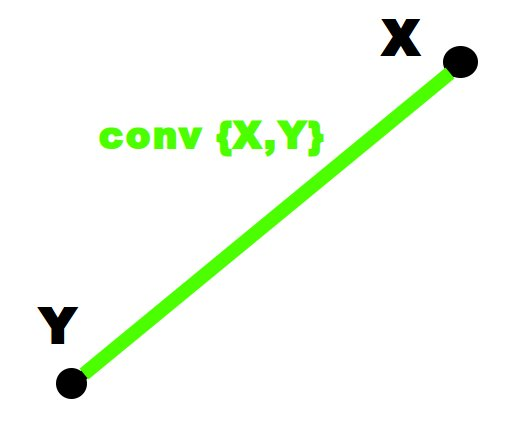
\includegraphics[scale=0.2]{./images/Course2_conv2}
\caption{Illustration of the convex hull of a set $X$. Note that the convex hull also includes the original set, wich is not very well represented on the figure.}
\label{conv}
\end{figure}

Taking the convex hull of the feasible set $X$ obviously gives us a new optimization problem. What are the optimal solutions of this new problem?\\

\begin{theorem}
Any optimal solution $x^*$ to the original problem :
$$\min_{x \in X} c^T x$$
is also optimal for the new problem :
$$\min_{x \in conv \: X} c^T x$$
\end{theorem}

This also means that the \textit{optimal values} of the two problems are the same. But because $X \subseteq conv \: X$, some optimal solutions of the new problem won't be in the original set $X$. So, in order to find the original optimal solutions, once we have solved the convex problem, we should always reject the optimal solutions of the new problems that aren't in $X$. Mathematically speaking : 
$$\{x^*_{original\,problem}\} = \{x^*_{new\,convex\,problem}\} \cap X $$

So, to summarize, we can make \textit{every problem in the world} convex, and we can (not yet, but after finishing this course) solve convex problems with good algorithms! This implies that basically any optimization problem can be solved easily! It seems too good to be true, and it is, since there is a \textbf{catch}\label{catch}. Although the definition of complex hull is rather simple, taking the convex hull of a general (that is, a little sophisticated) set is a very difficult operation.

So, in general, this approach is useless. There are specific cases, however, where this can be very useful!

The first, is a special case of linear optimization with \textbf{or} constraints. In such a problem, the admissible set is the union of (possibly disjoint) polyhedra. Computing the convex hull of the union of polyhedra can be done very efficiently, if the vertices are known, since the only task is to compute the vertices that will stay extreme in the union. The figure \ref{fig:my_label} illustrates this example.

\begin{figure}[H]
\centering
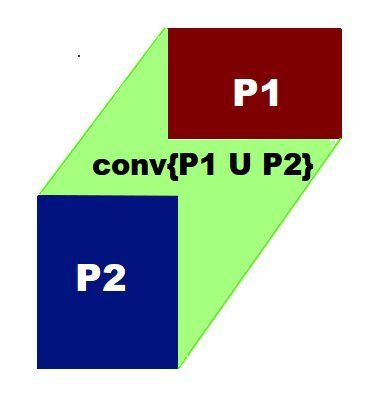
\includegraphics[scale=.4]{./images/Course2_polynoms}
\caption{Two (simple) disjoint polyhedron and the convex hull (in green) of the union.}
\label{fig:my_label}
\end{figure}

An interesting point to be raised here, is that such a problem could also be solved by computing the solution on every polyhedron, then choosing the best one. For small problems, this is of course valid, but for high number of dimensions, the cost of solving the problem on each polyhedron becomes prohibitive, while computing the convex hull remains a relatively cheap operation. 

The second case where taking the convex hull is useful is for (some) discrete models. Indeed:
$$\begin{array}{ccl}
\min_{x_i \in \{-1,1\}} c^T x & \Longleftrightarrow & min_{x} c^T x  \\
 & & -1 \leq x_i \leq 1
\end{array}$$

The convex hull of $\{-1,1\}^n$ is $[-1,1]^n$, and so both problems have the same solutions. The flow problem with integers (as seen in LINMA1702), which retains integer only solutions with relaxation, is an example of taking the convex hull of discrete problems without changing the nature of solutions. 

\subsection{Approximate \textit{any} convex problem by a linear problem}

It is possible to approximate convex problems by linear ones. Since the objective can always be converted to a linear function by adding a variable, the only work to be done concerns the constraints. Basically, the idea is to approximate the (closed\footnote{Why not open? Because an open set corresponds to strict inequalities, which cannot and will not be treated with the common optimization tools (see ``A note on $\neq$'', page \pageref{note_on_diff})}) set $X$ by a finite intersection of half-spaces (thus, linear constraints).

The way to do this is to use \textbf{projections} of points on the convex space. The projection of a point $u$ on a set $X$ is defined as the point $u_p \in X$ that minimizes the distance between itself and $u$.\\

\begin{theorem}{\textbf{Uniqueness and existence of projection.}}
Let $X$ be a \textbf{closed, non-empty, convex} set in $\mathbb{R}^n$, the projection of any exterior point on $X$ exists and is unique.
\end{theorem}

It is easy to see that the closeness and non-emptiness guarantee the existence of such projection. The unicity, however, is ensured by the convexity of the set. As an example, it is easy to see that a non-convex set such as the unit circle as an infinite number of projections of the origin.


With this concept of projection, we can introduce the \textbf{separation property}: for every exterior point $u$ of a convex closed set $X$, there exists a plane that \textit{separates} $u$ from $X$, that is, such that every element of $X$ is on \textit{one side} of the plane, while $u$ is on the \textit{other side}. This results directly from the uniqueness and existence of the projection of $u$ on $X$, although this was not demonstrated in class. Intuitively, this separation plane can be built perpendicular to the segment joining $u$ and its projection, without intersecting the convex plane.

So, to approximate a convex set by a linear one, the following method should be applied: for every point that should not be in $X$, create a separation plane. Such plane defines a half-space containing all of $X$. The intersection of all the half-spaces obtained this way forms a polyhedron containing $X$.

Moreover, it is interesting to note that an infinite number of points will create the convex set itself! This yields a new definition for a convex set: a convex set can always be written as the infinite intersection of half-spaces. This definition also proves immediately that every polyhedra is convex.

\begin{figure}[H]
\centering
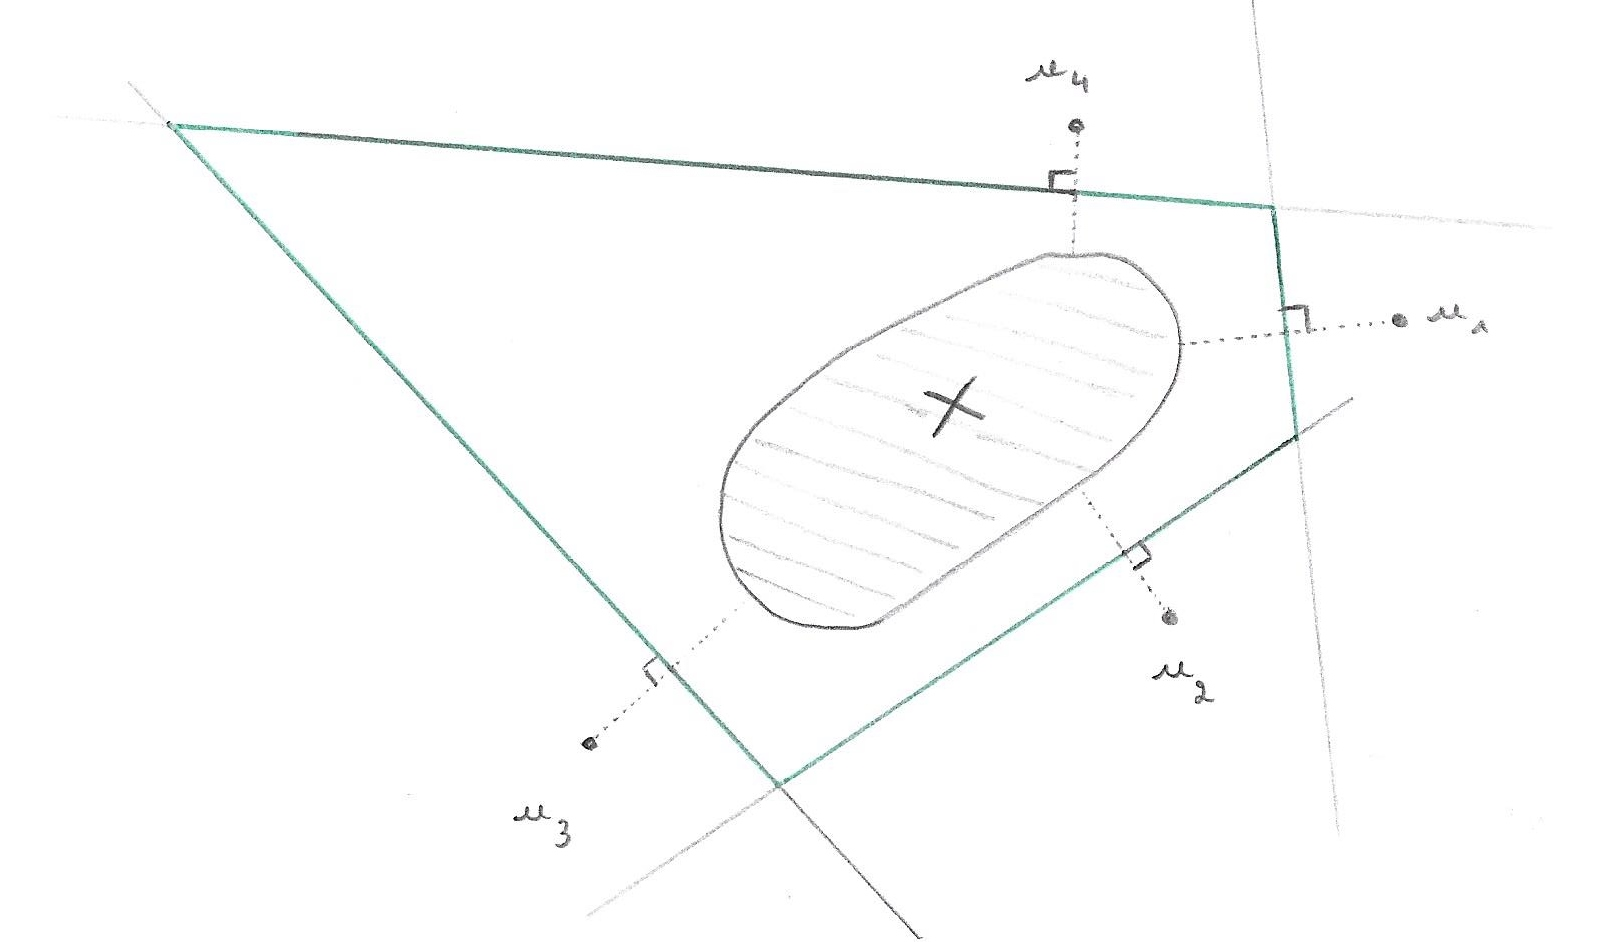
\includegraphics[scale=.4]{./images/Course2_Scan}
\caption{Approximation of a non-linear problem by a linear one.}
\label{labello}
\end{figure}
%\end{document}


%\documentclass{article}
%\usepackage[utf8]{inputenc}
%\usepackage{graphicx}
%\usepackage{amsmath}
%\usepackage{amssymb}
%
%\title{\textbf{LINMA2471: Optimization II - Models and Methods \\
%Course Notes - 30th September 2015}}
%\author{CHIEM Benjamin - 2174 1200\\
%GERARD Céline - 2590 1200 \\
%HAVELANGE Andine - 2583 1200 }
%\date{October 2015}
%
%\begin{document}
%
%\maketitle

\section{Modelling Tricks}

After studying the standard form of some optimization problems, we will see some model\-ling tricks which permit to transform a non-linear or non-convex problem into a linear or convex optimization problem. 

\subsection{Monotonicity}

\begin{definition}
A monotonic function over an interval is a function that is either increasing or decreasing over this interval.
\end{definition}

The transformation that is described in the following lines uses monotonic functions to turn an optimization problem into a simpler one. These operations do not change the problem but can change the solution and the optimal value of the objective of the problem. Let's see some examples.

\begin{example}
\begin{leftbar}
$\min \; \|x\|_{2}$ with $x \in X$ is equivalent to $\min \; \|x\|_{2}^{2}$ with $x \in X$. In fact, $z \rightarrow z^2$ is a monotonic function (increasing in this case) over $\mathbb{R}$. By solving this problem, we will find the same optimal solution than the first model but the value of the objective function will be different.
\end{leftbar}
\end{example}

\begin{example}
\begin{leftbar}
These functions are monotonic and can be used like in the previous example to simplify the problem:
\begin{itemize}
\item[.]{$z \rightarrow e^z$}
\item[.]{$z \rightarrow \log(z), \; (z>0)$}
\item[.]{$z \rightarrow -\frac{1}{z}, \; (z>0)$ for example, we can change $\min \; \frac{1}{\|x\|_{2}}$ to $\min \; -\|x\|_{2}$}\\
\end{itemize}
\end{leftbar}
\end{example}

We not only use this trick to modify the objective function, but also some constraints. For example: 
$$f(x) \leq b \Leftrightarrow e^{f(x)} \leq e^{b}$$
\begin{example}
\begin{leftbar}
\textbf{Advertisement for bank account:}
This example allows us to look at the effects of monotonicity in real life optimization problems.
We put money into an account where we can't take our money back sooner than 5 years after. The bank guarantees that we have a high percentage when we take back our money after 5 years and assures the three rates over 3 years given on Figure \ref{ra}.\\ 
What is the worst global rate compatible with this? Therefore, we are looking for the cumulative effect of the 5 rates (given over a year). 

\begin{center}
  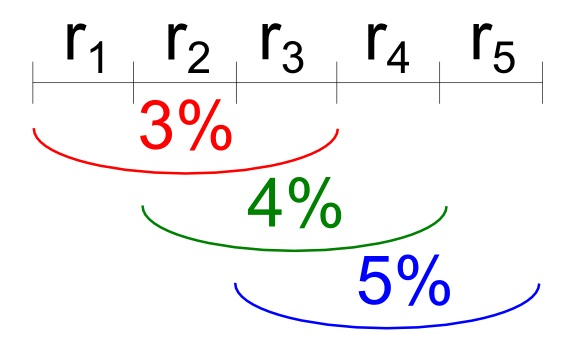
\includegraphics[scale=0.3]{./images/Course3_rate.jpg}
  \captionof{figure}{Rates}\label{ra}
\end{center}

To solve this problem, we introduce the variables $r_i$ corresponding to the rate per year where $i = 1,...,5$. We don't want a rate which is negative or null so we have the following optimization problem:
$$\min \limits _{r_i > 0} r_1r_2r_3r_4r_5 $$
under the constraints: 
$$ r_1r_2r_3 \geq 1.03$$
$$ r_2r_3r_4 \geq 1.04$$
$$ r_3r_4r_5 \geq 1.05$$

This problem is not linear. We can transform it into a linear problem if we use the logarithm function. Indeed, let $y_i = \log(r_i) \; \forall i=1,...,5$. We can do this because the logarithm is a monotonic increasing function. The problem can be written as: 
$$ \min \; y_1 + y_2 + y_3 + y_4 + y_5$$
under the constraints: 
$$ y_1 + y_2 + y_3 \geq \log(1.03)$$
$$ y_2 + y_3 + y_4 \geq \log(1.04)$$
$$ y_3 + y_4 + y_5 \geq \log(1.05)$$
This problem is now linear (and thus convex). \\

\textbf{Remark}: If we don't make the change of variable $y_i = \log(r_i) \; \forall i=1,...,5$,  the variables $r_i$ appear in $\log$ so the problem isn't linear.
\textbf{Remark}: The solution is surprising: it can be shown that the problem is unbounded! Take for example $y1=-M$, $y2=-M$, $y3=2*M+10$, $y4=-M$, $y5=-M$ which is feasible for any value of $M$, and whose objective value $10-2*M$ can be as negative as we want.


\end{leftbar}
\end{example}

\subsection{Change of variables}

We use change of variables in order to transform the problem into a linear or convex problem. For example, if every variable appears in a logarithm, then we can use the change of variable to remove the logarithm.\\ 
\textbf{Remark}: every appearance of the variables needs to match the change of variables! \\

For example, signomials\footnote{A signomial is an algebraic function of one or more variables of the form:\\ $f(x_1,x_2,...x_n) = \sum_i{(c_i\prod_j{x_j^{a_{ij}}})}$ where $c_i >0$.} can be converted into convex functions thanks of this trick. Let's consider the signomial $\frac{x_1x_2^2}{x_3^{\frac{1}{2}}}$. Let $x_i = e^{y_i}$, we obtain the following expression by change of variable $e^{y_1+2y_2-\frac{1}{2}y_3}$. Moreover, the exponential of a linear function is convex and the change of variables conserves the convexity (see later \textcolor{red}{Should add correct reference}).

\subsection{Misleading/Deceptive appearances}

In this part, we are looking for a polynomial $p(x), \; x \in \mathbb{R}$ of degree $D$ which fulfils some characteristic (see Figure \ref{poly}): 
\begin{itemize}
\item{For $x \in \left[0;f_1\right]$, $p(x) \geq 3$}
\item{For $x \in \left[f_2;f_3\right]$, $p(x) \leq 0.5$} \\
\end{itemize}

Let $p(x) = \sum_{i=0}^{D} a_i x^{i}$.
On the Figure \ref{poly}, we observe that the polynomial will not be linear or convex. We then have the impression that the optimization problem is not linear. But it is not the case, given that the variables are not the $x_i$ but the $a_i$.
Furthermore, the constraints (2 examples of constraints are given below) are linear. 
$$ \sum_{i=0}^{D} a_i 50^{i} \geq 3 \Leftrightarrow p(50) \geq 3$$
$$ \sum_{i=0}^{D} a_i 100^{i} = 1 \Leftrightarrow p(100)=1$$

\begin{figure}[ht!]
\centering
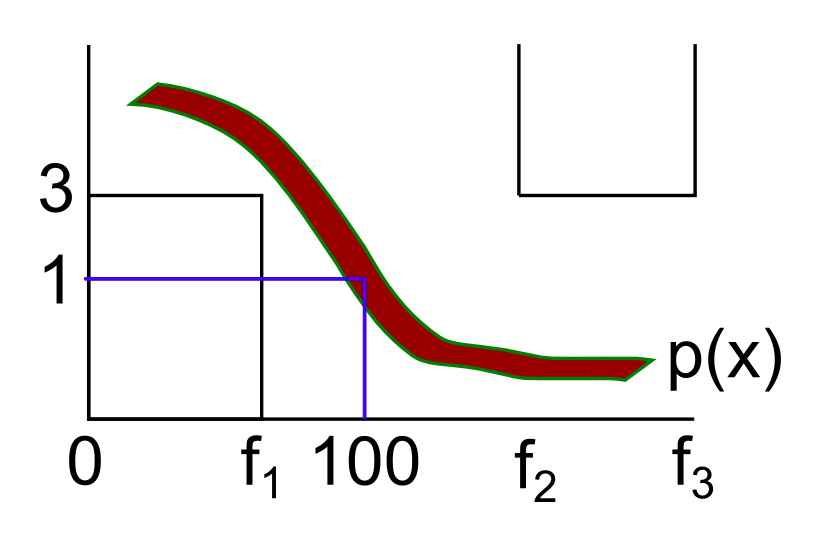
\includegraphics[scale=0.4]{./images/Course3_poly.png}
\caption{Polynomial $p(x)$}
\label{poly}
\end{figure}

\subsection{Flexibility}
The flexibility of an optimization problem is its capacity to be solved in different ways depending on which criterion we really want to optimize. Let us consider an approximation problem. We have a set of points $(x_i,y_i)$ in $\mathbb{R}^2$, and we want to find the function (which is often a polynomial) which approximates \textit{at best} these points. In other words, we want to find a function $f$ that minimizes the errors $\epsilon _i$ at the approximation points:
\begin{eqnarray*}
\epsilon_i &=& |y_i - f(x_i)|
\end{eqnarray*}
The question now is to choose the way to minimize errors $\epsilon _i$. Indeed, we could choose to minimize overall errors with a least square criterion: 
\begin{eqnarray*}
\min ||\epsilon||_2 &=& \sqrt{\sum_i{\epsilon_i^2}}
\end{eqnarray*}
Another choice would be to minimize the sum of the errors:
\begin{eqnarray*}
\min ||\epsilon||_1 &=& \sum_i{|\epsilon_i|}
\end{eqnarray*}
Finally, a last (often used) way to minimize errors is to minimize the maximum error: 
\begin{eqnarray*}
\min\;\max_i \epsilon_i
\end{eqnarray*}
All these considerations prove that, depending on the criterion we choose to optimize (i.e. depending on the context), the result could be different. For example, the problem
\begin{eqnarray*}
\max &\textnormal{safety}&\\
\textnormal{cost} &\le& m
\end{eqnarray*}
will not lead to the same solution than
\begin{eqnarray*}
\min &cost&\\
safety &\ge& b
\end{eqnarray*}

\subsection{Charnes and Cooper}

Consider the non-linear problem which is a division of two linear expression: 
$$ \min \; \frac{c^{T}x + d}{f^{T}x + g}$$
under the constraints: 
$$ Ax \leq b$$

In this case, taking the logarithm of the objective function will not change anything: we will have the same problem. \\

We make the hypothesis that $f^{T}x+g > 0 \; \forall x \textnormal{ such that } Ax \leq b$. If not, we have the solution $-\infty$ which is not an interesting solution. \\

To solve this problem and make it linear, we are going to homogenize the objective function. Let $x = \frac{y}{t}$ with $y \in \mathbb{R}^{n}$ and $t >0 \in \mathbb{R}$. If we take $t=1$ then we get back to the original problem. So, one solution in $x$ correspond to several solutions in $(y,t)$ (for example: $(x,1), \; (2x,2), \; ... \; (\lambda x,\lambda)$).\\
We can write the problem as: 
$$ \min \; \frac{\frac{c^{T}y}{t}+d}{\frac{f^{T}y}{t}+g} $$
with: 
$$ A\frac{y}{t} \leq b$$

By simplification, we obtain the following problem: 
$$ \min \; \frac{c^{T}y + dt}{f^{T}y + gt}$$
with:
$$Ay \leq bt$$

Now, we notice that the objective function's numerator and denominator are linear as the constraint. This problem has a property called homogeneity. If you take any solution, you can multiply any component by the same constant and nothing changes. Mathematically:\\
$(y,t)$ solution $\Rightarrow (\lambda y, \lambda t)$ solution $\forall \lambda \neq 0$ \\

We are going to choose solutions satisfying: $f^{T}y+gt=1$. We can do this using the property of homogeneity. This step results in selecting one solution among the collection of solutions multiple of each other. The objective function gets simpler and linear and we add one constraint. So, we have the following linear optimization problem: 
$$ \min c^{T}y + dt$$
with: 
$$ Ay-bt \leq 0$$
$$f^{T}y+gt = 1$$
$$t \geq 0$$

We compute $y^{*}$ and $t^{*}$ from this problem and take $x^{*} = \frac{y^{*}}{t^{*}}$ the solution of the original problem.\\ 
\textbf{Remark}: If we have $t=0$ at the optimum then the problem is unbounded and $x^{*} \rightarrow \infty$ (see Example \ref{unbounded}).\\
\begin{example}
\label{unbounded}
\begin{leftbar}
$$ \min \; \frac{1}{x}$$
with: 
$$x \geq 1$$ 

This problem have an optimal value of 0 so the solution $x^{*} \rightarrow + \infty$. 
\end{leftbar}
\end{example}

\section{Convex Optimization: Theorems and properties}
\subsection{Convex sets}

\subsubsection{Definition and examples}
\begin{definition}
A set X is convex if and only if
$$x,\;y \in X \Rightarrow \lambda x +(1-\lambda )y \in X \;\;\; \forall \; 0 \le \lambda \le 1$$
\end{definition}

Thus, a set is convex if and only if it contains all the segments joining any pair of its points.

\begin{example}
\begin{leftbar}
Here are several examples:
\begin{itemize}
\item $\mathbb{R}^n$, $\mathbb{R}^n_+$, $\emptyset$
\item Hyperplans ($\{x|\; b^Tx=\beta\}$)
\item Open or closed half-spaces ($\{x|\;b^Tx<\beta\}$ and $\{x| \;b^Tx\le \beta\}$)
\item Open and closed balls ($\{x|\;\|x-a\|<r\}$ and $\{x|\;\|x-a\|\leq r \}$)
\end{itemize}
\end{leftbar}
\end{example}

\subsubsection{Properties}
\begin{property}
Given a collection of convex sets $\{C_i\}_{i \in I} \subseteq \mathbb{R}^n$ ($I$ can be arbitrary), then $\bigcap \limits _{i \in I}C_i$ is convex too.
\end{property}
It follows that polyhedrons are convex because they are intersection of half-spaces.\\

\begin{property}
Given a collection of convex sets $C_1,\; C_2,\; C_3,\; ....\;C_n$, their cartesian product $C_1\times C_2 \times C_3 \times ... \times C_n$ is convex too. 
\end{property}
\vspace{0.5cm}
\begin{property}
If $X\subseteq \mathbb{R}^n$ and $X\subseteq \mathbb{R}^n$ are convex then the Minkowski sum of $X$ and $Y$, $X+Y=\{x+y\;|\;x \in X \;\text{and} \; y \in Y\}$ is convex too. 
\end{property}

\textbf{Remark}: The union of convex sets is not always convex!

\subsection{Convex functions}
\subsubsection{Definition and examples}
\begin{definition}
A function f with domain D is a convex function of and only if \\
\begin{center}
D is convex and 
\end{center}
$$x,y\; \in D \Rightarrow f(\lambda x+(1-\lambda)y) \le \lambda f(x)+(1-\lambda)f(y) \;\;\; \forall \; 0\le \lambda \le 1$$
\end{definition}
\vspace{0.5cm}
\begin{example}
\begin{leftbar}
Here are several examples:
\begin{itemize}
\item Linear and affine functions are convex ($x \rightarrow \alpha x$,  $x\rightarrow b^Tx$  and  $x \rightarrow b^Tx+\alpha$)
\item The norm function and the square of the norm function are convex functions ($x \rightarrow \|x\|$ and $x \rightarrow \|x\|^2$)
\item Quadratic forms ($x \rightarrow x^TQx$) are convex functions when the matrix $Q \in \mathbb{R}^{n\times n}$ is semi positive definite
\item The functions $x \rightarrow e^x$,  $x\rightarrow -log(x)$ and $x \rightarrow |x|^p \;\;(1 \le p)$ are convex
\end{itemize}
\end{leftbar}
\end{example}
\vspace{0.5cm}
\begin{definition}
A function $f$ is concave $\Leftrightarrow$ $-f$ is convex.
\end{definition}

\textbf{Remark}: Linear and affine functions are convex and concave.

\subsubsection{Properties}

To know whether a function is convex or not, we have to transform it into its epigraph and check if it is convex or not. But there are some useful properties of convex functions that we can use to spare time. 
\vspace{0.5cm}
\begin{property}
If $f$ is a convex function and $c \in \mathbb{R}_0^+$, then $cf$ is convex.  
\end{property}
\vspace{0.5cm}
\begin{property}
If $f$ and $g$ are convex functions, then $f+g$ is convex. 
\end{property}
\vspace{0.5cm}
\begin{property}
Given a collection of convex functions $\{f_i\}_{i \in I}: \mathbb{R}^n \rightarrow \mathbb{R}$, $\sup \limits _{i \in I}f_i$ is convex too.\\
With $\left[ \sup \limits _{i \in I} f_i\right] (x)= \sup \limits _{i \in I} f_i(x)$
\end{property}
\vspace{0.5cm}
\begin{property}
Given $f(x,s)$ (with $x \in \mathbb{R}^n$ and $s \in \mathbb{R}$, a parameter) such that $x \rightarrow f(x,s)$ is convex for any $s$, 
$$\int_{s \in S}f(x,s)ds\;\; \text{is \;convex}$$
\end{property}

\subsection{Properties of convex functions}
\subsubsection{Convexity and differential calculus}

\begin{property}
Let $f$ be a differentiable function of which the domain D is open. 
$f$ is convex if and only if D is convex and
$$\forall x,y \; \in D, \;f(y)\geq f(x)+\nabla f(x)^T(y-x) $$
\end{property}
This property means that, if $f$ is convex, it will be above all its Taylor approximations of first order. This signifies that at any point, the tangent of the function is under the function. This is useful to make a piecewise approximation of $f$ by linear functions (an example of such an approximation is shown on Figure \ref{ApproximationConvexe}). In order to obtain such an approximation, we have to choose $n$ points at which we calculate the tangent of the function $f$ and then take the maximum of the $n$ tangents (in the example, $n=3$). \\
Besides, the value of the approximation is lower than the real value on any point. It allows us to obtain lower bounds.\\

\begin{figure}[ht!]
\centering
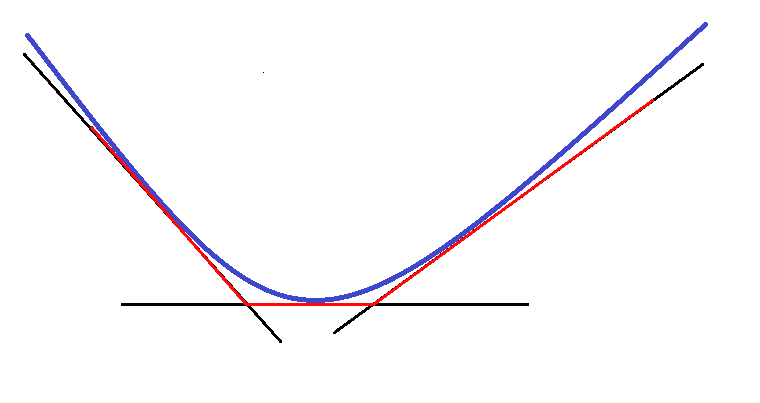
\includegraphics[scale=0.4]{./images/Course3_ApproximationConvexe.png}
\caption{Illustration of the piecewise linear approximation of a convex function}
\label{ApproximationConvexe}
\end{figure}

\begin{property}
Let $f$ be a twice differentiable function of which the domain D is open. 
$f$ is convex if and only if D is convex and
$$\forall x\in D,\; \nabla^2f(x)\geq 0 $$
\end{property}


\subsubsection{Convexity and linear transformations}
Linear transformations preserve convexity. Indeed,
\vspace{0.5cm}
\begin{property}
If $S\subseteq \mathbb{R}^n$ is convex and $\Phi: \; \mathbb{R}^n \rightarrow \mathbb{R}^m: \; x \rightarrow Ax+b$ is a linear transformation, then the image of $S$ by $\Phi$,
$$\Phi (S)=\{\Phi(x)|\; x \in S\}$$
is convex too. 
\end{property}
\vspace{0.5cm}
\begin{property}
If $\Phi: \; \mathbb{R}^n \rightarrow \mathbb{R}^m: \; x \rightarrow Ax+b$ is a linear transformation and $f:x\rightarrow f(x)$ is a convex function, then
the composition 
$$f\circ \Phi=f(\Phi(x))=f(Ax+b)$$
is convex too. 
\end{property}
\vspace{0.5cm}
\begin{property}
If $S\subseteq \mathbb{R}^n$ is convex and $\Theta: \; \mathbb{R}^m \rightarrow \mathbb{R}^n: \; x \rightarrow ax+b$ is a linear transformation, then
the image of $S$ by the inverse of $\Theta$,
$$\Theta ^{-1} (S)=\{x|\;\Theta (x) \in S\}$$
is convex too. 
\end{property}

%\documentclass[12pt,a4paper]{article}
%\usepackage[utf8]{inputenc}
%\usepackage[english]{babel}
%\usepackage{amsmath, amsthm, amssymb}
%\usepackage{array}
%\usepackage{graphicx}
%\newtheorem{property}{Proposition}
%\newtheorem{example}{Example}[section]
%\newtheorem{remark}{Remark}
%\newtheorem{property}{property}
%\newtheorem{defi}{Definition}
%\usepackage{float}
%\usepackage{graphicx}
%\usepackage[left=2cm,right=2cm,top=2cm,bottom=2cm]{geometry}
%\title{LINMA2471: Optimization models and methods: course 4 \\
%\begin{center}
%(07/10/2015)
%\end{center}}
%\author{Adissa Laurent, Laura Motte and Caroline Sautelet}
%\begin{document}
%\maketitle
% \section{Properties of convex functions}
% \subsection{Linear transformation on the variables}
\vspace{0.5cm}
\begin{property}
 Given a convex and affine transformation $ x \mapsto Ax + b $, the composition $x \mapsto f(Ax + b)$ is also convex.
 \end{property}
 \begin{example}
\begin{leftbar}
	$e^{2x - y + z}$ is convex because the exponential is convex and  $2x - y + z$ is a linear transformation of $x, y$ and $z$.
	\end{leftbar}
	\end{example}
	
  \begin{example}
\begin{leftbar}	
	\textbf{Convex functions}\\
	Any norm $x \mapsto ||x ||$ is convex, thus the distance $||x-y||$ between two points $x$ and $y$ is convex because $x-y$ is a linear transformation.\\
    The maximum distance between a set $S$ and a point $x$ is a convex function. Indeed, taking the maximum between a point and a set requires to take the maximum of all the distances between the point and any point in the set (distance between two points is a convex function): $f_{S,max} = \max_{s \in S}\{ ||x - s|| \}$ 
	\end{leftbar}
	\end{example}
	%\begin{remark}
	%The minimum distance between a convex set $S$ and a point $x$ is convex: $f_{S,max} = \min_{s \in S} ||x - s||$
	%\end{remark}
    
    \subsubsection{Partial minimization}
    
    \begin{property}\label{partialmin}(Partial minimization)
    If the function $f: (x,y) \mapsto f(x,y) $ is convex, then $f_x (y) = \inf_{x} f(x,y) $ is convex.
\end{property}

\begin{example}
\begin{leftbar}
If a set S is convex, then the minimum distance function between a point x and the set S is convex. Indeed, one can write the function as follow:
$$f(x,s) = ||x-s||$$
Since this is a norm, f is convex. Since the restriction of a convex function stays convex as long as the feasible region stays convex and S is a convex set, property \ref{partialmin} gives that:
$$ f_S(x) = \inf_{S} f(x,s)$$ 
is a convex function.
\end{leftbar}
\end{example}
    
\textbf{Remark}: Property \ref{partialmin} is a one side property. A counter-example for the reverse side is given by:
$$f_x(y) + \sqrt{||x||}$$

\subsubsection{Extended real valued functions}

Most of theorems to prove the convexity of a function require the convexity of the domain. However, it is possible to extend a function to tackle this problem. 

\begin{example}
\begin{leftbar}
Let's take the function $f: \mathbb{R}_+ \mapsto \mathbb{R}: x \mapsto \frac{1}{x}$ and extend it such that its domain becomes the whole real line. One consider: 
$$f_e: \mathbb{R} \mapsto \mathbb{R} \cup \{ + \infty \}: x \mapsto 
\begin{cases} \frac{1}{x} \text{ if } x > 0 \\
+ \infty \text{ elsewhere}
\end{cases}$$
One can see that the extended function is convex over the whole real line. The epigraph definition still holds since there isn't any point above $+\infty$.
\end{leftbar}
\end{example}

\subsubsection{Composition and product}
\begin{property}
If $g$ is a convex function and $h$ is a convex, increasing and one-dimensional function then the composition function $h \circ g: x \mapsto h(g(x))$ is also convex. 
\end{property}
\begin{proof}
Let's prove this proposition for a simple case. We assume that $h$ and $g$ are both one-dimensional functions and that $h,g \in \mathcal{C}^2$. The general case requires a more difficult proof. \\
Since f and g are 2 times differentiable, one has:
$$\big[ h(g(x))\big]'' = \big[ h'(g(x))g'(x)\big]' = \underbrace{h''(x)(g'(x))^2}_\text{A} + \underbrace{h'(g(x))g''(x)}_\text{B} $$

Since h is convex, its second derivative is positive and given that a square is positive, one has that $A$ is positive. Furthermore, since $g$ is also convex and $h$ is increasing, one also has that $B$ is positive. One conclude that the second derivative of $h \circ g$ is positive and thus, the function $h \circ g$ is convex. 
\end{proof}
\textbf{Remark}: Sometimes we need to square a value but also to keep convexity (for example, we don't care about negative deviations on a budget) \textcolor{red}{Should be better expressed}. However the traditional square function is not convex \textcolor{red}{(increasing??)} on the real line. Let's introduce a restricted square function as follows: 
$$f: x \mapsto (x_+)^2 = (\frac{x + |x|}{2})^2$$
We easily see (Figure \ref{restricted}) that this restricted square function is convex.

\begin{figure}[H]
\begin{center}
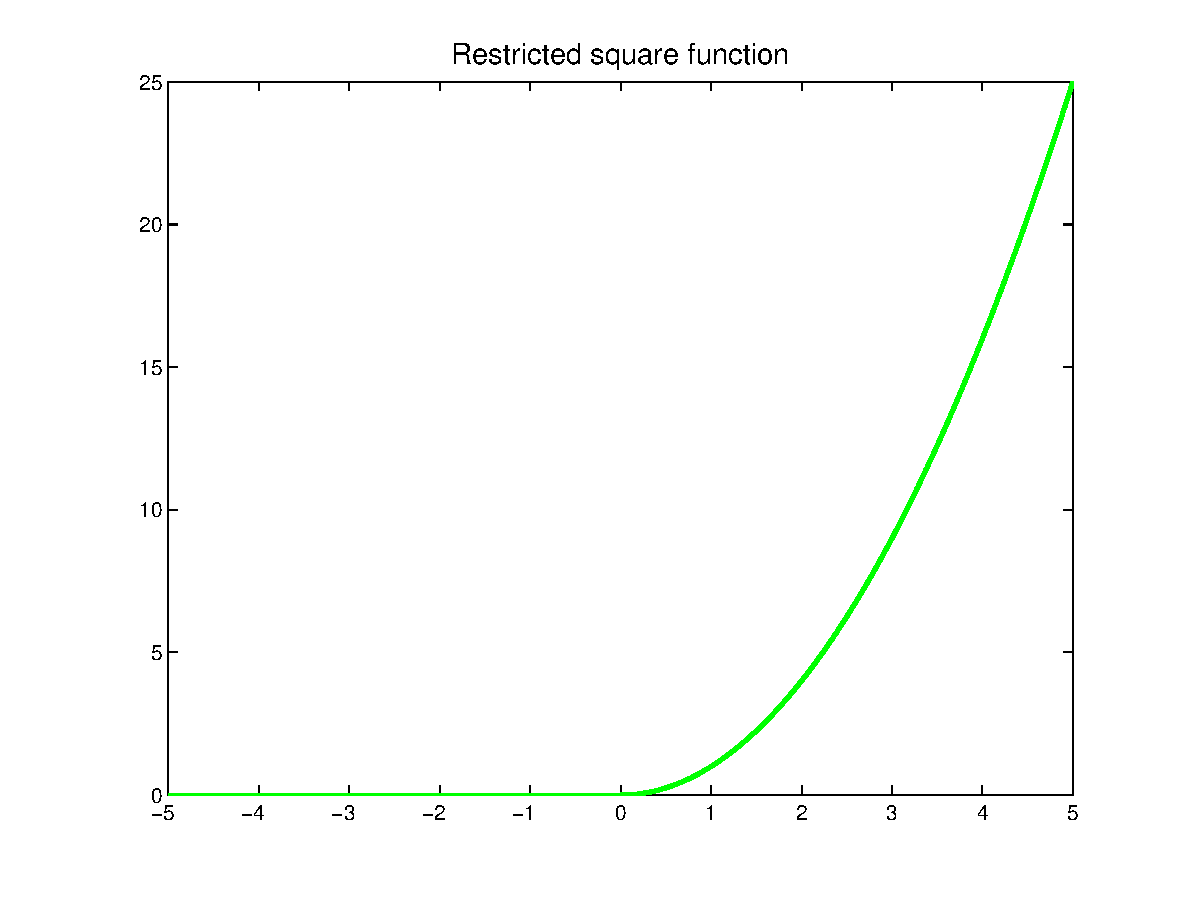
\includegraphics[scale=0.5]{./images/Course4_restrictedsquare.eps}
\caption{Restricted square function}
\label{restricted}
\end{center}
\end{figure}

\begin{example}
\begin{leftbar}
The function $\big[ \log(x+y)_+\big]^2$ is convex. Indeed, the restricted square \textcolor{red}{(is convex and increasing???)} and $-\log$ are convex functions. Therefore, their composition is convex. Since $x+y$ is a linear transformation, it preserves convexity and the whole function is convex. 
\end{leftbar}
\end{example}
\vspace{0.5cm}
\begin{property}\label{product}
If f and g are both convex, positive and increasing then their product is convex.
\end{property}
\begin{proof}
Again, one proves it in the simple differentiable, one-dimensional case. 
One has:
$$(fg)'' = \big[ f'g + fg'\big]' = f''g + 2f'g'+fg''$$
The result follows immediately since by assumptions one has $f,g,f',g',f'',g'' \geq 0$.  
\end{proof}
\textbf{Remark}: The previous proof tends to indicate variants of Property \ref{product}. One can see that if $f$ and $g$ are both concave, decreasing and negative then the proposition still holds.  

\subsection{Advantage of convex problems}
\begin{property}
Let's recall that $ \min_{x \in X} f(x)$ is convex if $f$ is convex, $X$ is convex and we are looking for a minima. We study the properties of a convex problem:
\vspace{0.5cm}
\begin{center}
 \begin{tabular}{p{7cm}|p{7cm}} 
    MODEL & METHODS \\
    \hline
	  & \\
  - Local minima are also global & - Methods which only work on convex problems: first order, second order...  \\
   - The set of optimal solutions is convex & \\
	& \\
    - Using duality we can get guarantees & \\
 \end{tabular}
 \end{center}

 \end{property}
 \subsection{Variants of convex functions}
 It's a difficult thing to know if a problem has a unique solution. There is one class of problems with only one solution: minimization of strictly convex functions.
 \vspace{0.5cm}
 \begin{definition}
 Strict convexity: $f$ is strictly convex if and only if 
 \begin{itemize}
 \item The domain is convex
 \item $f(\lambda x + (1-\lambda)y)<\lambda f(x) + (1-\lambda) f(y)$ $\forall x,y \in \textnormal{Dom}$ , $\forall \lambda \in ]0,1[$
 \end{itemize}
 \end{definition}
\vspace{0.5cm}
 \begin{example}
 \begin{leftbar}
 On the following graph, we can observe that the function is strictly convex.
 \begin{center}
 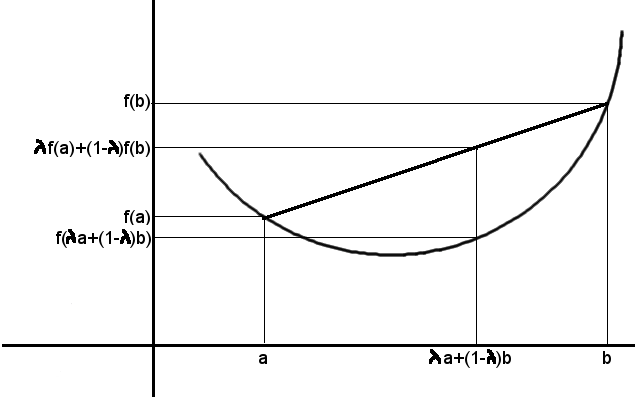
\includegraphics[scale=0.4]{./images/Course4_courbe}
 \end{center}
 \end{leftbar}
 \end{example}
\vspace{0.5cm}
\begin{example}
\begin{leftbar}
The absolute function is not strictly convex. In fact, when we have a flat part in the graph, it can not be strictly convex.
\begin{center}
  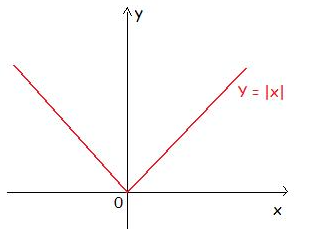
\includegraphics[scale=0.5]{./images/Course4_absolue}
\end{center}
\end{leftbar}
\end{example}
\vspace{0.5cm}
\begin{example}
\begin{leftbar}
The function $x \mapsto ||x||_{2} = \sqrt{\sum_{i} x_{i}^{2}}$ is convex but not strictly convex.
\end{leftbar}
\end{example}
\vspace{0.5cm}
\begin{property}
If we have $\min f(x)_{x \in X}$ with $f$ strictly convex and $X$ a convex set then the problem admit at most one solution.
\end{property} 
\vspace{0.5cm}
\begin{property}
If $ f \in C^{2}$ and $\nabla^{2} f(x) > 0 $ then $f$ is strictly convex. ($\lambda_{i} > 0 $ $\forall i$)
\end{property}
\vspace{0.5cm}
\begin{property}
If $f$ is convex, then $ f + ||x||^{2}_{2}$ is strictly convex.
\end{property}
\begin{proof}
Assume $f \in C_2$ 
\\then $$\nabla^{2}(f + ||x||^{2}) = \nabla^{2} f  + \nabla^{2}||x||^{2}_{2} = \nabla^{2} f + 2I
$$
where $||x||_{2}^{2} = \sum_{i} x_{i}^{2}$ and $\lambda_{i} \geq 0$.
\end{proof}
\vspace{0.5cm}
\begin{property}
$$(1) \ \lambda \text{ is an eigenvalue of } M$$
$$\Leftrightarrow$$
$$(2) \ \lambda + \Delta \text{ is an eigenvalue of } M + \Delta I$$
\\for any $\Delta \in \mathbb{R}$ and $M \in \mathbb{R}^{n \times n}$ symmetric.
\end{property}
\begin{proof}
$$ (1) \ \exists v \: \ M v = \lambda v $$
$$(2) \ \exists v \: \ (M + \Delta I) v = ( \lambda + \Delta)v$$
\end{proof}
\textbf{Remark}: We can have the same propositions and the same proof while adding $\mu > 0$ anywhere: $ f + \mu ||x||^{2}$. It is a regularization to make it strictly convex.\\
\textbf{Remark}: There are functions that have no derivative and are strictly convex.
	
\chapter{First-order methods}
\label{Ch2}

%\documentclass[a4paper, 11pt]{article}
%\usepackage[cm]{fullpage}
%\usepackage[english]{babel}
%\usepackage[latin1]{inputenc}
%\usepackage[T1]{fontenc}
%\usepackage{color}
%\usepackage{ulem}
%\usepackage{fancyvrb}
%\usepackage{amsmath}
%\usepackage{amsfonts}
%\usepackage{graphicx} 
%\usepackage{xcolor}
%\usepackage{listings}
%\usepackage{textcomp}
%
%\usepackage{tikz}
%\usepackage{circuitikz}
%\usepackage{pgfplots}
%\usepackage{graphicx}
%\usetikzlibrary{calc,through,backgrounds}
%\usetikzlibrary{decorations.markings,decorations.pathmorphing,decorations.pathreplacing}
%\usetikzlibrary{arrows,shapes,positioning}
 %\tikzstyle arrowstyle=[scale=1]
 %\tikzstyle directed=[postaction={decorate,decoration={markings,
    %mark=at position .5 with {\arrow[arrowstyle]{stealth}}}}]
 %\tikzstyle reverse directed=[postaction={decorate,decoration={markings, 
   %mark=at position .5 with {\arrowreversed[arrowstyle]{stealth};}}}]
%\usepackage{rotating}
%\usepackage{multirow}
%\pgfplotsset{compat=1.10}
%
%\newcounter{examplecounter}
%\newenvironment{example}{\begin{quote}
    %\refstepcounter{examplecounter}
  %\textbf{Example \arabic{examplecounter}}
  %\quad}{\end{quote}}
%
%\newcounter{lemmacounter}
%\newenvironment{lemma}{\begin{quote}
    %\refstepcounter{lemmacounter}
  %\textbf{Lemma \arabic{lemmacounter}}
  %\quad}{\end{quote}}
%
%\newcounter{propcounter}
%\newenvironment{proposition}{\begin{quote}
    %\refstepcounter{propcounter}
  %\textbf{Proposition \arabic{propcounter}}
  %\quad}{\end{quote}}
%
%\title{LINMA2471 - Optimization\\
%Cours 5}
%\author{S. \textsc{Cheng}, Q. \textsc{Le}, F. \textsc{Delcourt}}
%\date{\today}
 %
 %
%\begin{document} 
%\maketitle


We've been investing in convex models and trying to find the best formulation of optimization problems. We now explore different methods that allow us to solve those problems and study their properties. In this part we focus on first order methods. Second order methods will be discussed further.

\section{Gradient Method}

A main example of first order methods is the Gradient Method also known as the Steeped Descent Method. Many practical problems have constraints but let's consider for the moment that we have none.  
 
Problem:  $\underset{x  \in \mathbb{R}^n}{\text{min }} \: f(x) $
 
\begin{lstlisting}[mathescape,caption=Gradient Algorithm]
Given $x_0$, $k=0$
Repeat
$x_{k+1} = x_k - \underbrace{h_k}_{\in \mathbb{R}} \underbrace{\nabla f(x_k)}_{\in \mathbb{R}^n}$
$k \leftarrow k+1$
\end{lstlisting}

$h_k$ is called the step length and $-\nabla f(x_k)$ is called the direction.


\section{Step length selection}

\subsection{ $h_k$ that minimize $f(x_k - h_k \nabla f(x_k))$} 

We have to solve for $h_k$ at each step. Even if we only minimize one variable, it's still an iterative method and does not give directly $h_k$. 

\subsection{$h_k = \alpha$}

\begin{example}\begin{leftbar}
Let's consider $x^2$ and see what happens when we change $h_k$

\framebox[1.5cm][c]{$h_k = 2$} $\quad \forall k$ \\
Set $x_0$ \\
$x_1 = x_0 - 2(2x_0) = -3x_0$\\
$x_2 = -3x_0 - 2(-6x_0) = 9 x_0$\\
Instead of going to zero we go to $-3x_0$ or $9x_0$. Our step is clearly too large. This is called DIVERGING.

\framebox[1.5cm][c]{$h_k = 1$} $\quad \forall k$ \\
$x_1 = x_0 - 2x_0 = -x_0$\\
$x_2 = = -x_0 - (-2x_0) = x_0$ \\
This time, we are still too large and this is called CYCLING. 

\framebox[1.5cm][c]{$h_k = \frac{1}{2}$} $\quad \forall k$ \\
$x_1 = x_0 - \frac{1}{2}(2x_0)$ = 0 \\
We have a FINITE CONVERGENCE. 

\framebox[1.5cm][c]{$h_k = \frac{1}{3}$} $\quad \forall k$ \\
$x_1 = x_0 - \frac{1}{3}(2x_0) = \frac{1}{3}x_0$\\
$x_2 = \frac{1}{3}x_0 - \frac{1}{3}(2\frac{1}{3}x_0) = \frac{1}{9}x_0$\\
$\vdots$\\
$x_k = \frac{1}{3^k}x_0$ \\

We get closer to $x_0$. 

\end{leftbar}\end{example}

The simple gradient method is subjected to poor step length selection. However it still good to use a constant step length. We'll explicitly and numerically compute some value of $\alpha$ which guarantee a good behavior. 

\subsection{$h_k$ satisfies some "dynamic" conditions (e.g. Wolfe condition)}

In order to know what is the best step length, we need to know the function. We focus only on functions that are $C_L^{1,1}$, which means that $f \in C^1$ and $\nabla f$ is Lipschitz with constant L. The Lipschitz condition is:
$$\| \nabla f(x) - \nabla f(y) \| \leq L \| x-y \|$$
In order words, if we take 2 points, their gradient can't be too different.\\

Mathematically, we can define: 

\begin{definition}
Given $L>0$, we say $f : D \subseteq \mathbb{R}^n \to \mathbb{R}$ has \emph{$L$-Lipschitz gradient} if and only if $f \in C^1(D)$ and
\begin{equation*}
\vnorm{\nabla f(x) - \nabla f(y)} \le L \vnorm{x-y}
\end{equation*}
for all $x,y \in D$. We denote $C_L^{1,1}(D)$ the set of such functions. We also define
\begin{equation*}
F_L^{1,1}(D) = \{ f \in C_L^{1,1}(D) \mid f \text{ is convex}\} .
\end{equation*}
\end{definition}

Given $f \in C^1$, we also denote $T^1_y(x) = f(y) + \nabla f(y)^T (x-y)$ the first-order Taylor expansion of $f$ around $y$ evaluated at point $x$.


\begin{example}\begin{leftbar}
Function that are Lipschitz with L=0? Linear function are $C_0^{1,1}$
\end{leftbar}\end{example}

\begin{example}\begin{leftbar}
Standard quadratic function $x \rightarrow x^T Q x $  with no convexity assumption for now. The Lipschitz condition can be expressed as: 
$$ \| 2Qx - 2Qy \| \leq L \| x-y \|  \quad \forall x,y$$
$$ 2 \| Q (x -y)  \| \leq L \| x-y \| \quad \forall x,y$$
If $Q=Id$, it's clear that $L = 2$.  When it comes to matrix like Q, we will use the spectral norm. From the matrix theory, we  know that:
$$ \| Qv \|_2 \leq \underbrace{\| Q\| _2}_{max \vert \lambda_i (Q) \vert} \| v \|_2$$

One can hence choose $$L=2 \| Q \|_2 $$

For more complicated function, we can try to bound the value of L  and use  its estimate. 
\end{leftbar}\end{example}

As we can see, it's very easy to compute the constant for a quadratic function. But what can we do in a more  general case?\\

\begin{property} 
When f  $ \in C^2$ the Lipschitz constant is given by $ L=\underset{x}{\text{max }} \| \nabla^2 f(x) \|$ .
\label{5:prop1}
\end{property}
This result is very useful for one variable functions but not for multi-variables functions. The computation can be hard in that case.

\begin{example}\begin{leftbar}
Let's apply proposition \ref{5:prop1} with $f: x \rightarrow \sqrt{1+x^2}$
\begin{eqnarray*}
f'(x)=& \frac{x}{\sqrt{1+x^2}}\\
f''(x)=& \frac{ \sqrt{1+x^2}-x \frac{x}{ \sqrt{1+x^2}}}{1+x^2}=\frac{1}{(1+x^2)(\sqrt{1+x^2})}\\
\end{eqnarray*}  
We easily see that:
$$ 0 \leq \frac{1}{(1+x^2)(\sqrt{1+x^2})} \leq 1$$
The upper bound is clear and we also put the lower bound because we want the absolute value of $f''(x)$ to be bounded. We  will take $L=1$.
\end{leftbar}\end{example}

What can we say about the minimum of a function based only on its first derivative? We are tempted to use the Taylor series which approximate the function by its tangent.  Unfortunately  we can't say anything from this about the minima. One better idea is to construct an upper bound approximation of our function using the Lipschitz constant then try to minimize this bound. We are thus sure that our function will stay below this bound, as shown in Figure \ref{5:fig1}. 

\begin{figure}[H]
\begin{center}
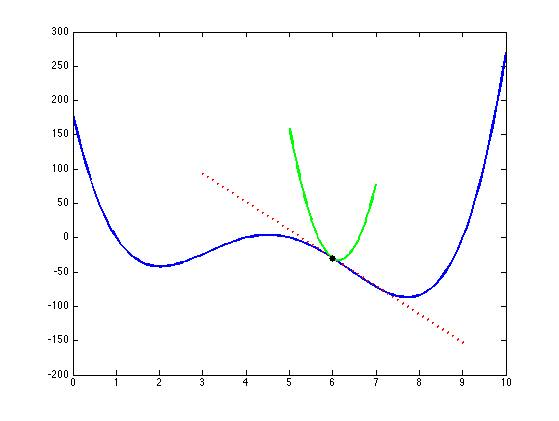
\includegraphics[scale=0.6]{./images/Course5_construction} 
\caption{In blue: $f$ of $C_L^{1,1}$, in red: tangent to the function, in green: the QUB}
\label{5:fig1}
\end{center}
\end{figure}

\begin{lemma}
\textbf{Quadratic upper bound (QUB) of $C_L^{1,1}$ function} \\
Let's $f \in C_L^{1,1}$. Then for any $x$ we have that 
$$ \hat{f}: y \mapsto  f(x)+ \nabla f^T(x)(x-y)+ \frac{L}{2} \| x-y\|^2 $$
 is an upper bound of $f(y)$.
\end{lemma}

Notice that $\hat{f}$ is a quadratic function of $y$.  What is the minimum of the quadratic upper bound? Our function is now convex and easy to minimize over $y$.


$$\nabla \hat{f}(y)=0 \Leftrightarrow  \nabla f(x) +\frac{L}{2} 2(x-y)(-1)=0$$

$$ \Rightarrow y^{*} = x- \frac{1}{L} \nabla f(x)$$

We can notice that the last equation is very similar to the gradient method. It is sensible to use $h_k=\frac{1}{L}$ in our method. 

\subsection{Analysis of the $h_{k}$= $\frac{1}{L}$ gradient method}
 
After one step, taking  $y= x-\frac{1}{L}\nabla f(x)$, the upper bound gives:
\begin{align*}
\hat{f}(y)=f(x) + \nabla f(x)^{T} [\frac{-1}{L} \nabla f(x)]+\frac{L}{2} \|  \frac{-1}{L}\nabla f(x)\|^2
& =f(x)- \frac{\|\nabla f(x)\|^{2}}{L}+\frac{1}{2L} \|\nabla f(x)\|^{2} \\
& =f(x)-\underbrace{\frac{1}{2L} \|\nabla f(x)\|^{2}}_{\leq 0}
\end{align*}
Looking at all iterations now:
$$ f(x_{k+1})-f(x_{k}) \leq - \frac{\|\nabla f(x_k)\|^{2}}{2L}$$
(because the upper bound displays this decrease \textcolor{red}{What does it mean?})\\


$f(1)-f(0) \leq -\dfrac{\|\nabla f(x_{0})\|^{2}}{2L}$\\
$f(2)-f(1) \leq -\dfrac{\|\nabla f(x_{1})\|^{2}}{2L}$ \\
$\vdots$ \\
$f(N+1)-f(N) \leq -\dfrac{\|\nabla f(x_{N})\|^{2}}{2L}$\\

Summing the equations above, we get \\
$f(N+1)-f(0) \leq - \dfrac{1}{L} \sum\limits_{i=1}^{N+1}$ $\|\nabla f(x_{i})\|^{2}$\\
so we deduce \\
$2L(f(0)-f(N+1)) \geq \sum\limits_{i=1}^{N+1} \|\nabla f(x_{i})\|^{2} \geq (N+1) \min \|\nabla f(x_{i})\|^{2}$

Hence
\begin{align*}
\underset{i=0,...,N}{\text{min }} \|\nabla f(x_{i})\| & \leq \sqrt{\frac{2L(f(0)-f(N+1))}{N+1}} \\
& \leq \sqrt{\frac{2L(f(0)-f(x^*))}{N+1}}
\end{align*}
with $x^*$ minimum point of $f$.

\begin{lemma}
Assume in addition that $f$ is convex (meaning $f \in F^{1,1}_{L}$)\footnotemark, then we have: 
$$ f(N)-f(x^*) \leq \frac{L\|x_{0}-x^*\|^{2}}{2N} $$ 
 (assuming $x^*$ is one of the minimum points).
\end{lemma}
\footnotetext{$f$ is convex and $f \in C_{L}^{1,1}$}
 
\begin{example}\begin{leftbar} Behaviour of the gradient method
$$2x^{2}+y^{4}-2y^{2}$$
we start from (1,0)

 \begin{equation*}
   \nabla=
 \begin{pmatrix}
4x  \\
4y^{3}-4y
\end{pmatrix}
\end{equation*}

\begin{equation*}
   \nabla^{2}=
 \begin{pmatrix}
4 & 0 \\
0 & 12y^{2}-4
\end{pmatrix}
\end{equation*}
We have three stationary points $(0,0)$,$(0,1)$,$(0,-1)$. 

We observe that
 \begin{equation*}
   \nabla(1,0)=
 \begin{pmatrix}
4  \\
0
\end{pmatrix}
\end{equation*}
If we start from $(1,0)$, we can only converge to $(0,0)$ and we couldn't find all the points. 
\end{leftbar}\end{example}








%\end{document}
	

%\documentclass{article}
%\usepackage[utf8]{inputenc}
%\usepackage{amsmath}
%\usepackage{amsthm}
%\usepackage{amssymb}
%\usepackage{enumitem}
%\usepackage[left=2.5cm,right=2.5cm,top=2.25cm,bottom=2.25cm]{geometry}
%\usepackage{multirow}
%
%\title{LINMA2471 -- Optimization models ans methods II \\ Notes from the $6^\mathrm{th}$ lecture}
%\author{Antoine Aspeel \and Pierre-Paul Mouchet \and Guillaume Olikier}
%\date{October 21, 2015}
%
%% Definitions and propositions
%\newtheorem{theorem}{Theorem}
%\newtheorem{prop}[theorem]{Proposition}
%\newtheorem{lemma}[theorem]{Lemma}
%\newtheorem{coro}[theorem]{Corollary}
%\theoremstyle{definition}
%\newtheorem{definition}{Definition}
%\newtheorem{ex}{Example}
%
%% Shortcuts

%
%
%
%\begin{document}
%
%\maketitle





\section{Gradient method for unconstrained problems}

\subsection{Gradient method for functions of $C_L^{1,1}$}

In the previous section, we studied the gradient method for the general problem.
\begin{equation*}
\min_{x \in \mathbb{R}^n} f(x)
\end{equation*}
where $f \in C_L^{1,1}(\mathbb{R}^n)$. We proved that $\frac{1}{L}$ was actually the best step length choice and that it guaranteed
\begin{equation}
\min_{0 \le i \le N} \vnorm{\nabla f(x_i)} \le \sqrt{\frac{2L(f(x_0)-f(x^*))}{N+1}} .
\label{MinGrad}
\end{equation}
Observe that this inequality
\begin{itemize}
\item is scaling independent,
\item doesn't say anything about the values of $f$.
\end{itemize}
One can show that this inequality is not improvable. \\

Let us recall the way we obtained the above inequality.

\begin{lemma}[Quadratic bounds in $C_L^{1,1}$]
The following conditions are equivalent :
\begin{enumerate}% [label=(\alph*)]
\item $f \in C_L^{1,1}(D)$,
\item $f \in C^1(D)$ and $|f(y) - T_x^1(y)| \le \frac{L}{2}\vnorm{x-y}^2$ $\forall x,y \in D$.
\end{enumerate}
\label{qbCL}
\end{lemma}
\begin{proof}
See the fourth exercises session.
\end{proof}

From this lemma, we concluded that $\frac{1}{L}$ is the optimal step length.

\begin{theorem}[Decrease guarantee]
Let $f \in C_L^{1,1}$. Denote $x^+ = x - \frac{1}{L}\nabla f(x)$ the next iterate. Then
\begin{equation*}
f(x) - f(x^+) \ge \frac{{\vnorm{\nabla f(x)}}^2}{2L}.
\end{equation*}
\label{DecreaseGuar}
\end{theorem}
\begin{proof}
Use the upper bound of lemma \ref{qbCL} with $y = x^+$.
\end{proof}
\noindent Actually there exist a family of functions which can be as closed of this bound as you want. \\

Finally theorem \ref{DecreaseGuar} leads to the inequality \eqref{MinGrad}.

\subsection{Gradient method for functions of $F_L^{1,1}$}

Let us now consider the same problem with the additional assumption $f \in F_L^{1,1}(\mathbb{R}^n)$. Lemma \ref{qbCL} can be improved as follows.

\begin{lemma}[Quadratic bounds in $F_L^{1,1}$]
The following conditions are equivalent :
\begin{enumerate}%[label=(\alph*)]
\item $f \in F_L^{1,1}(D)$,
\item $f \in C^1(D)$ and $T_y^1(x) \le f(x) \le  T_y^1(x) + \frac{L}{2}\vnorm{x-y}^2$ for all $x,y \in D$.
\end{enumerate}
\label{qbFL}
\end{lemma}
\begin{proof}
See the fourth exercises session.
\end{proof}

\begin{lemma}
Let $f \in C_L^{1,1}$. For any optimal solution $x^*$ and any $x$,
\begin{equation*}
\frac{{\vnorm{\nabla f(x)}}^2}{2L} \le f(x) - f(x^*) \le \frac{L}{2} {\vnorm{x-x^*}}^2 .
\end{equation*}
\end{lemma}
\begin{proof}
The first inequality follows from theorem \ref{DecreaseGuar} since $f(x^+) \ge f(x^*)$. The second inequality follows from lemma \ref{qbCL} applied with $x = x^*$. Indeed since $f \in C^1$ and $x^*$ is a local extremum, we have $\nabla f(x^*) = 0$.
\end{proof}

\begin{theorem}[Convergence of $\frac{1}{L}$-gradient method for $F_L^{1,1}$]
Let $f \in F_L^{1,1}$. For any iterate $x_N$ and any $x_0$,
\begin{equation*}
f(x_N) - f(x^*) \le \frac{L}{2N} \vnorm{x_0-x^*}^2 .
\end{equation*}
\end{theorem}
\begin{proof}
We start from theorem \ref{DecreaseGuar}:
\begin{equation*}
f(x^+) \le f(x) - \frac{{\vnorm{\nabla f(x)}}^2}{2L} .
\end{equation*}
Since $f \in C^1$ and $f$ is convex, we have
\begin{equation*}
f(x^*) \ge f(x) + \nabla f(x)^T(x^*-x),
\end{equation*}
right-hand side being tangent equation around $x$. Combining these two inequalities yields
\begin{equation*}
f(x^+) \le f(x^*) + \nabla f(x)^T(x-x^*) - \frac{1}{2L} {\vnorm{\nabla f(x)}}^2 .
\end{equation*}
Now, observe that\footnote{Apply $\vnorm{a-b}^2 = \vnorm{a}^2 - 2a^Tb + \vnorm{b}^2$ to $a = x-x^*$ and $b = \frac{1}{L}\nabla f(x)$. Ok, it's a trick.}
\begin{equation*}
\nabla f(x)^T(x-x^*) - \frac{1}{2L}{\vnorm{\nabla f(x)}}^2 = \frac{L}{2} \left( \vnorm{x-x^*}^2 - \vnorm{x-x^*-\frac{1}{L}\nabla f(x)}^2 \right) .
\end{equation*}
Noting that $x-\frac{1}{L}\nabla f(x) = x^+$, we obtain
\begin{equation*}
f(x^+) - f(x^*) \le \frac{L}{2} \left( \vnorm{x-x^*}^2 - \vnorm{x^+-x^*}^2 \right) .
\end{equation*}
So given $N \in \mathbb{N}$, we have for all $i \in \{0,...,N-1\}$
\begin{equation*}
f(x_{i+1}) - f(x^*) \le \frac{L}{2} \left( \vnorm{x_i-x^*}^2 - \vnorm{x_{i+1}-x^*}^2 \right) .
\end{equation*}
Summing those $N$ inequalities yields
\begin{align*}
\sum_{i=0}^{N-1}f(x_{i+1}) - N f(x^*) &\le \frac{L}{2} \sum_{i=0}^{N-1}\left( \vnorm{x_i-x^*}^2 - \vnorm{x_{i+1}-x^*}^2 \right) \\
&= \frac{L}{2} \left( \vnorm{x_0-x^*}^2 - \vnorm{x_N-x^*}^2 \right) \\
&\le \frac{L}{2} \vnorm{x_0-x^*}^2 .
\end{align*}
Notice now that $f(x_N) \le f(x_i)$ for all $i \in \{0,...,N-1\}$ so that
\begin{equation*}
 N f(x_N) \le \sum_{i=1}^Nf(x_i) .
\end{equation*}
Using this in the last inequality, we finally get
\begin{equation*}
f(x_{N}) - f(x^*) \le  \frac{L}{2N} \vnorm{x_0-x^*}^2 . \qedhere
\end{equation*}
\end{proof}

Among all methods with
\begin{equation*}
x_k \in \myspan\{x_0, \nabla f(x_0), ..., \nabla f(x_{N-1})\},
\end{equation*}
none of them can guarantee better than
\begin{equation*}
f(x_N) - f(x^*) \le \frac{3}{32}L \frac{{\vnorm{x_0-x^*}}^2}{(N+1)^2}
\end{equation*}
for dimension greater or equal to $2N+1$.

\section{Gradient method for constrained problems}

We now add constraints. We consider problems of the following form:
\begin{equation*}
\min_{x \in C} f(x) \qquad \text{with} \quad f \in C_L^{1,1}(C)
\end{equation*}
and
\begin{equation*}
\min_{x \in C} f(x) \qquad \text{with} \quad f \in F_L^{1,1}(C) .
\end{equation*}
We assume $C \subseteq \mathbb{R}^n$ is a convex and closed set. This implies that the orthogonal projection on $C$
\begin{equation*}
P_C : \mathbb{R}^n \to C : x \mapsto P_C(x)
\end{equation*}
is well defined and unique.\\

\begin{definition}
Let $\mathcal{C}$ be a closed convex set and f a differentiable function ($f \in C_L^{1,1}(C)$), we say that $x^*$ is a \textbf{stationary point} of the problem $\min\limits_{x \in C} f(x)$ if and only if
\begin{equation*}
\langle \nabla f(x^*), x-x^* \rangle \ \geq\ 0 \ \ \ \ \forall x \in C
\end{equation*}
\end{definition}
This definition can be intuitively interpreted as follows: adding $f(x^*)$ on both sides brings up the first-order Taylor expansion of $f$ around $x^*$, which is closed to $f(x)$. So this definition essentially means $f(x) \ge f(x^*)$.\\
In another interpretation, that means that all possible errors $x-x^*$ are in opposite direction with $-\nabla f$. A schema of the situation is shown on figure \ref{tik1}.
\begin{figure}[H]
\centering
\begin{tikzpicture}
\draw (0,0) circle (1);
\draw[fill = black] (1,0) circle (0.05);
\draw (0,-1.3) node{$C$};
\draw (1.2,-0.2) node{$x^*$};
\draw[>=latex,->] (1,0) -- (2,0) node{$\ \ \ \ \ \ \ \ \ \ -\nabla f$};
\draw[>=latex,->] (1,0) -- (1.866025403784439,0.5);
\draw[>=latex,->] (1,0) -- (0,0);
\draw[>=latex,->] (1,0) -- (0.133974596215561,0.5);
\draw[>=latex,->] (1,0) -- (0.133974596215561,-0.5);
\draw[>=latex,->] (1,0) -- (0.4,0.8);
\draw[>=latex,->] (1,0) -- (0.4,-0.8);
\draw[red] (1.5,0.15) -- (1.3,0.35);
\draw[red] (1.35,0.1) -- (1.45,0.4);
\end{tikzpicture}
\caption{Example of a stationnary point $x^*$.}
\label {tik1}
\end{figure}

\begin{example}
\begin{leftbar}
 $C = \{x \in \mathbb{R}^n: x_i \ge 0\}$ (nonnegative orthant)
\begin{align*}
&x^* \; \text{stationnary iff} \; \sum_i \left[\nabla f(x^*)\right]_i \left[x_i - x_i^*\right] \ge 0\ \ \ \forall x\ge 0\\
&x^* \; \text{stationnary iff either} \; [\nabla f(x^*)]_i=0\\ 
&\phantom{x^* \; \text{stationnary iff eith}}\text{or} \; [\nabla f(x^*)]_i>0 \; \text{and} \; x_i^*=0 \; \forall \; i
\end{align*}
Indeed, as $\sum_i [x_i - x_i^*] \ge 0$ for all $x\ge0$,  $[\nabla f(x^*)]_i$ must be $\ge 0$.
If not, we could choose a very large $x_i$ for this component and have a negative sum.
\end{leftbar}
\end{example}

\begin{example}
\begin{leftbar}
It also works easily for $C = \{x|\sum_{i}x_i=1\}$ which is a kind of budget constraint. In that case, it is possible to show that $[\nabla f(x^*)]_i = \lambda \; \forall i$. That means that all the gradient components are equal to each other, or economically speaking that the marginal costs are equal to each other. At the optimum, the marginal cost is equal for each component, it does not matter which one you lower.
\end{leftbar}
\end{example}

\begin{example}
\begin{leftbar}
(not treated) The Euclidian bowl.
\end{leftbar}
\end{example}


Note that if $x^* \in \myint\, C$, then necessarily $\nabla f(x^*) = 0$.
Indeed, if $\nabla f(x^*) \neq 0$ and $x^* \in \myint\, C$, we can choose $x$ such that $\nabla f(x^*)$ and $x-x^*$ are of opposite directions. Consequently, their scalar product is negative which contradicts the definition of $x^*$. This implies that $\nabla f(x^*) = 0$.

\begin{theorem}
Under the above assumptions, if $x^*$ is a local minimum, then $x^*$ is stationary.
\end{theorem}

\begin{theorem}
When $f$ is convex, stationary implies optimality.
\end{theorem}


\subsection{Projected gradient method}
Let us now present the gradient method for constrained problems. The principle is the following:
\begin{enumerate}
\item at each step, minimize the quadratic upper bound on set $C$,
\item which is equivalent to projecting the true minimum of the quadratic upper bound on set $C$.
\end{enumerate}
Let us show this equivalence. Statements mean
\begin{enumerate}
\item choose $x^+$ minimizing $f(x) + \nabla f(x)^T(x^+-x) + \frac{L}{2}{\vnorm{x-x^+}}^2$ over $C$, where we can ignore the constant term $f(x)$ in the minimization problem,
\item choose $x^+$ minimizing ${\vnorm{x^+ - (x - \frac{1}{L}\nabla f(x))}^2}$ over $C$. Notice that we can develop
\begin{equation*}
\begin{array}{rcl}
\vnorm{x^+ - (x - \frac{1}{L}\nabla f(x))}^2 & = & \vnorm{(x^+ - x) + \frac{1}{L}\nabla f(x))}^2 \\
& = & \vnorm{x^+-x}^2 + \dfrac{2}{L}(x^+-x)^T \nabla f(x) + \dfrac{1}{L^2} \vnorm{\nabla f(x)}^2
\end{array}
\end{equation*}
which is equivalent to 1 since we can ignore the constant term $\vnorm{\nabla f(x)}^2/L^2$ and multiply by $L/2$ without changing the minimization problem.
\end{enumerate}

This results in the following algorithm.

\begin{lstlisting}[mathescape,caption=Projected gradient method]
Given $x_0,L,k=0$ 
Repeat
$\qquad  x_{k+1} = P_C(x_k - \frac{1}{L}\nabla f(x_k))$
$\qquad  k \leftarrow k+1$
\end{lstlisting}


% \end{document}
	

%\documentclass[a4paper]{article}
%\usepackage[utf8]{inputenc}
%\usepackage{amsthm}             % Definitions and such
%\usepackage{amssymb}            % R for space and such
%\usepackage{amsmath}
%\usepackage[a4paper]{geometry}
%
%\title{LINMA2471 : Optimization models and models : course 6 (28/10/2015)}
%\author{Renaud Dufays, Antoine Durviaux \& Leïla Van Keirsbilck}
%\date{Octobre 2015}
%
%\usepackage{natbib}
%\usepackage{graphicx}
%\usepackage{framed}
%\usepackage{tikz}
%\usepackage{float}
%\usetikzlibrary{arrows}
%\usetikzlibrary{decorations.markings}
%
%
%\begin{document}
%
%\maketitle

\subsection{Gradient mapping for constrained problems}

\begin{definition}
For some $M>0$, the \textbf{gradient mapping} $G_M^Cf(x)$ is the unique vector satisfying 
\begin{equation*}
x - \frac{1}{M}G_M^Cf(x) = P_C\left[x - \frac{1}{M}\nabla f\right]
\end{equation*}
\end{definition}

The role of the gradient mapping is similar to the one of the gradient in the non-constraint case. Notice that if we take $\mathcal{C} = \mathbb{R}^n$, then $G_M^{\mathbb{R}^n}f(x) = \nabla f(x)$. An illustration of the gradient mapping is given in Figure \ref{tik2}.

\begin{figure}[H]
\centering
	\begin{tikzpicture}
    \draw (0,0) circle (1);
    \draw (0,-1.3) node{$\mathcal{C}$};
    \draw[>=latex,->, blue] (0.5,-0.5) -- (1.5,0);
    \draw[blue] (1.3,-0.5) node{$-\nabla f$};
    \draw[red] (0.4,0.1) node{$G_M^C f$};
    \draw[>=latex,->,red] (0.5,-0.5) -- (1,0);
    \draw[dashed] (1,0) -- (1.5,0);
    \draw (4,0) circle (1);
    \draw (4,-1.3) node{$\mathcal{C}$};
    \draw[>=latex,->, blue, dash pattern= on 3pt off 5pt] (3.5,-0.2) -- (3.5,0.5);
		\draw[>=latex,->, red, dash pattern= on 3pt off 5pt,dash phase=4pt] (3.5,-0.2) -- (3.5,0.5);
    \draw[blue] (4.4,0.2) node{$-\nabla f$};
		\draw[red] (5.6,0.2) node{$G_M^C f$};
		\draw (5,0.2) node{$=$};
    \end{tikzpicture}
\caption{Illustration of gradient mapping.}
\label {tik2}
\end{figure}

% \draw[blue,dash pattern= on 3pt off 5pt] (0,0) |- (1,1) to[out=0,in=90] (2,0);
% \draw[red,dash pattern= on 3pt off 5pt,dash phase=4pt] (0,0) |- (1,1) to[out=0,in=90] (2,0);

The gradient method becomes, in the case of constraint problems :

\begin{lstlisting}[mathescape,caption=Gradient Method - Constrained Problem]
Given $x_0$, $L$, $k=0$
Repeat
$\qquad   x_{k+1} = P_C[x_k - \frac{1}{L}G_M^C f(x_k)]$
$\qquad  k \leftarrow k+1$
\end{lstlisting}


\begin{property}
For any $M>0$, we have $x^*$ stationary iff $G_M^C f(x^*)=0$
\end{property}

\begin{property}
Given $f \in C^{1,1}_L$, and letting $x^+ = x - \frac{1}{L}G^C_L f(x)$ be the next step, we have
\[
    f(x) - f(x^+) \ge \frac{\left\|G_L^C f(x)\right\|^2}{2L}
\]
\end{property}


\begin{theorem} Using those properties, we obtain that for $f \in C_L^{1,1}$, the projected gradient method gives
\begin{equation*}
\min_{0\leq i \leq N} \left\|G_L^C f(x_i)\right\| \leq \sqrt{\frac{2(f(x_0) - f(x^*))}{L(N+1)}}
\end{equation*}
\end{theorem}

We have a stronger result in the case of a convex $f$, as stated by the following theorem.
\begin{theorem}
Let $f \in F_L^{1,1}$. For any iterate $x_N$ and any $x$,
\begin{equation*}
f(x_N) - f(x^*) \leq \frac{M\left\|x_0 - x^*\right\|^2}{2N}
\end{equation*}
\end{theorem}


The projected gradient method is quite slow because it is in $\mathcal{O}(\frac{1}{N})$ but also because projection can be complicated. Indeed, projection can be hard to compute if $\mathcal{C}$ is too complex.

\begin{example}
\begin{leftbar}
If $\mathcal{C}=\{x\ge0\}$ this is easy because $[P_C(x)]_i=\left\lbrace
\begin{array}{ll}
x_i & \mbox{if $x_i \ge 0$}\\
0 & \mbox{if $x_i < 0$}
\end{array}
\right.$
\end{leftbar}
\end{example}

\begin{example}
\begin{leftbar}
If $\mathcal{C}=\{x|Ax=b\}$ is a subspace, this is expensieve. We have indeed to solve a linear system, which is $\mathcal{O}(n^3)$.
\end{leftbar}
\end{example}

\begin{example}
\begin{leftbar}
If $\mathcal{C}=\{x|Ax\leq b\}$ is a polyhedron, this is even more expensive : the projection problem has to be written as a minimization of the distance (quadratic programming). We could also use a theorem that separates the problem on each facet of the polytope.
\end{leftbar}
\end{example}


\subsection{Acceleration gradient [Nesterov 1983]}


\begin{lstlisting}[mathescape,caption=Acceleration gradient]
Given $f \in C^{1,1}_L$, $x_0$, $L$, $k=0$ and $x_{-1}=x_0$
Repeat 
$\qquad y_k = x_k + \beta_k (x_k - x_{k-1})$
$\qquad x_{k+1} = P_C[y_k - \frac{1}{L}\nabla f(y_k)]$
$\qquad k \leftarrow k+1$
\end{lstlisting}

The first step is called an extrapolation step whereas the second is called a gradient step. Note that $y_k$ is not always in $\mathcal{C}$. The idea is to recycle the previous work because $(x_k - x_{k-1})$ will be close to the gradient.

\begin{theorem}
For $\beta_k=\frac{k-1}{k+2}$, we have
\begin{equation*}
f(x_N) -  f(x^*) \leq \frac{2L\left\|x_0 - x^*\right\|^2}{(N+1)^2}
\end{equation*}
\end{theorem}

It can be proved that this rate of $\frac{1}{N^2}$ is not improvable. Accelerated gradient is thus a sublinear method (slower than linear). While the gradient method is really robust, the accelerated method is extremely sensitive. Note that $\beta_k$ goes to 1 as $k$ goes to infinity. An example is the Huber function : on the linear part, the steps increase in a quadratic way.\\

\textbf{Linear convergence (to zero) :} $1, \rho, \rho ^2, \rho ^3, \rho ^4, \rho ^5, ... $ with $\rho < 1$. If we restrict the class of functions to \textbf{strongly convex}, we can get linear convergence.\\

\begin{definition}
Given $\mu>0$, f is $\mu$-\textbf{strongly convex} iff
\begin{equation*}
f(\lambda x + (1-\lambda)y)\leq \lambda f(x) + (1-\lambda)f(y) - \frac{\mu}{2}\lambda (1-\lambda)\left\|x - y\right\|^2
\end{equation*}
\end{definition}

A strongly-convex function can be viewed as a function that has no flat part.

\begin{proposition}
If $f \in C^2$ then f is $\mu$-strongly convex iff for all $x$ 
\[
    \lambda_{min}(\nabla^2f(x))\ge \mu
\]
\end{proposition}


\begin{lemma}
For any strongly convex function, we have
\begin{equation*}
\left\|x - x^*\right\|^2 \leq \frac{2}{\mu}[f(x) - f(x^*)]
\end{equation*}
That means that if I decrease the error on the function value, automatically I decrease the distance to the solution. Using previous results, we obtain :
\begin{equation*}
\left\|x_N - x^*\right\|^2 \leq \frac{2}{\mu}\frac{L\left\|x_0 - x^*\right\|^2}{2N} = \frac{L}{\mu}\frac{\left\|x_0 - x^*\right\|^2}{N}
\end{equation*}
\end{lemma}

$\frac{L}{\mu}$ is called the condition number.


\textbf{Remark:} The accelerated gradient method gives better results if we restart the method after a certain number of iteration. For example, if the squared norm of the error is divided by 5 after $N = 10$ iterations, it will be divided by 10 after $N = 20$ iterations. But if we restart the method after 10 iterations and make 10 new iterations, the square norm of the error will be divided by 25 although we made a total of 20 iterations in both cases. A result that is not proven here is that the optimal number of iterations after which the method should be restarted is $\frac{L}{\mu}\text{e}$. In this case, the method is linearly convergent and we have :
\[
    \left\|x_N - x^*\right\|^2 \leq \left(1-\frac{1}{\text{e}\frac{L}{\mu}}\right)\left\|x_0 - x^*\right\|^2
\]

%\end{document}
	
	
\chapter{Conic modelling and duality}

%\documentclass[10pt,a4paper]{article}
%\usepackage[utf8x]{inputenc}
%\usepackage[francais]{babel}
%\usepackage[T1]{fontenc}
%\usepackage{amsmath}
%\usepackage{verbatim}
%\usepackage{amsfonts}
%\usepackage{amssymb}
%\usepackage{graphicx}
%\usepackage{here}
%\usepackage{hyperref}
%\usepackage[left=2cm,right=2cm,top=2cm,bottom=2cm]{geometry}
%\newcommand{\HRule}{\rule{\linewidth}{0.5mm}}
%
%\usepackage{esvect} % Vecteurs
%\usepackage[amssymb]{SIunits}
%\usepackage{eurosym}
%\usepackage{mathrsfs}
%\usepackage{dcolumn}
%\usepackage{pifont}
%\usepackage{amsthm}
%
%
%%-------------------------------
%% TEST PACKAGES (GEO) POUR COMPILATION
%%-------------------------------
%\usepackage {lmodern}
%\usepackage{soul}
%\usepackage{fancyhdr} %un joli header
%\usepackage{enumerate}
%\usepackage{color}
%\usepackage{multicol}
%\usepackage{amsfonts}
%\usepackage{amsthm}
%\usepackage{mathrsfs}
%\usepackage{pifont}
%\usepackage{cancel}
%\usepackage{epstopdf}
%\usepackage{pifont}
%
%
%
%\title{CM7: LINMA 2471: Optimization methods and models: Lecture 7}
%\date{November, 4th 2015}
%\author{Ciamarra Geoffrey \and Losseau Bruno \and Lucas Joachim}
%
%\begin{document}
%\maketitle
%\selectlanguage{french}
%\theoremstyle{plain}
%\newtheorem{theorem}{Theorem}[section] % reset theorem numbering for each chapter
%\newtheorem{definition}{Definition}[section] % definition numbers are dependent on theorem numbers
%\newtheorem{example}{Example}[section] % same for example numbers
%
%\newtheorem{proposition}{Proposition}[section]
%\newtheorem{corollary}{Corollary}[section]
%\newtheorem{remark}{Remark}[section]

% Examples: \begin{example} .... \end{example}
% Definitions: \begin{definition} ... \end{definition}
% Theorems: \begin{theorem} ... \end{theorem}
% Propositions: \begin{proposition} ... \end{proposition}
% Remarks: \begin{remark} ... \end{remark}



\section{Conic optimization}
In order to introduce the conic optimization concept, let's begin with an linear example. 
\begin{example}[Linear optimisation problem]
\begin{leftbar}
\label{ex:C1}
\begin{align}
& & \nonumber \\ 
& \underset{y_i}{\max} \nonumber
& & 2y_1+3y_2+2y_3 \nonumber \\ 
& \text{subject to}
& & y_1 + y_2 \leq 1 \label{eq1} \\
& & & y_2 + y_3 \leq 2 \label{eq2} \\
& & & y_3 \leq 3 \label{eq3}
\end{align}

A feasible point is given by $(y_1,y_2,y_3)= (1,0,2)$ which provides a cost function value $6$. \\ \\ \textit{How to know whether $6$ is strictly lower than or strictly higher than or equal to the optimal objective value ?}  \\ \\ Since a feasible point gives $6$ as cost function value, the optimal objective value is not strictly lower than $6$. The value $6$ can be increased to $7$ by taking the feasible point $(y_1,y_2,y_3)= (2,-1,3)$. So the optimal objective value is not equal to $6$ but higher than $6$.\\ Concerning the value $7$, we could ask our question again,\textit{ how to prove that the optimal objective value is higher than or equal to $7$ ? } \\ \\ We need an upper bound on the value for the objective function. This can be achieved by taking a linear combination of the constraints. \\ \\ Indeed, 
\begin{align*}
2 \times \text{~constraint~} (\ref{eq1})+ 1 \times \text{~constraint~} (\ref{eq2})+ 1 \times \text{~constraint~}(\ref{eq3}) & = 2y_1+3y_2+2y_3 \\
& \leq 7
\end{align*}
$7$ is an upper bound for the objective value function. Since we have found a feasible point for which the objective value is equal to $7$, we can claim that the optimal objective value is equal to $7$. 
\end{leftbar}
\end{example}

It is possible to find a bound for the objective value for any linear problem. We want to extend the notion of linear problems while keeping their `nice' properties of linear problems (i.e. duality and efficient algorithms). In order to extend this notion, we will generalize the inequalities $\leq$ and $\geq$ in the linear problems. \\ \\
With $K \subseteq \mathbb{R}^n$, we define an generalized type of inequalities\[ a \succeq_K 0
 \Leftrightarrow a \in K \]
On the basis of this definition, we also have the following properties \begin{align*}
 a \succeq_K b \Leftrightarrow a-b \succeq_K 0
\Leftrightarrow a-b \in K \\ a \preceq_K b
\Leftrightarrow b \succeq_K a \Leftrightarrow b-a \succeq_K 0
\Leftrightarrow b-a \in K \end{align*}
Let us also impose two sensible properties for an order

\begin{property}
\label{Prop:C1}
$a \succeq_K 0 \Rightarrow \lambda a \succeq_K 0 \text{ for any } \lambda \ge 0$ 
\end{property}
\begin{property}
\label{Prop:C2}
$a \succeq_K 0 \text{ and } b \succeq_K 0 \Rightarrow a+b \succeq_K 0$
\end{property}
The Property \ref{Prop:C1} means that $K$ is a \emph{cone} and the Property \ref{Prop:C2} means that $K$ is \emph{closed under addition}.
The $K$ must be convex, $K$ is said to be a convex cone. In fact, for any cone $K$ (closed under non-negative scalar multiplication), we have the equivalence
\[ K \text{ is closed under addition } \Leftrightarrow K \text{ is convex} \]

\subsection{Generalization}
From the usual formulation of the problem, one can generalize: 
\begin{center}$\max b^Ty$ such that $A^Ty$ $\leqslant$ c \\
$\Downarrow$ \\
$\max b^Ty$ such that $A^Ty$ $\preceq_K$ c
\end{center}
This problem is convex.\\
Considering the standard linear case, $K = \mathbb{R}^n_+$.

\begin{example}
\begin{leftbar}
Going back to example \ref{ex:C1}, how would one define the set $K$?\\
As: 
\[A^T = \left( \begin{array}{ccc}
1 & 1 & 0 \\
0 & 1 & 1 \\
0 & 0 & 1 \end{array} \right), \hspace{1cm}
C = \left( \begin{array}{c}
1 \\
2 \\
3 \end{array} \right) \]
Defining $K = \mathbb{R}^3_+$ implies: 
\[C-A^Ty = 
\left( \begin{array}{c}
1 \\
2 \\
3 \end{array} \right)-
\left( \begin{array}{ccc}
1 & 1 & 0 \\
0 & 1 & 1 \\
0 & 0 & 1 
\end{array} \right) y
\subset K = \mathbb{R}^3_+ 
\]

\[\left( \begin{array}{c}
1 - y_1 - y_2 \\
2 - y_2 - y_3\\
3 - y_3 \end{array} \right) 
\subset K = \mathbb{R}^3_+ 
\]
\end{leftbar}
\end{example}

\subsection{Solving a problem on different cones}
As one consider polyhedron cones, the boundary is linear. Also, applying a linear operation to a linear problem keeps the problem linear. 
As a result, applying a rotation or a scaling operation to a cone and solving the problem on the newly obtained cone is equivalent to solving it on the first cone. \label{solving_diff_cones}
\begin{center}
\begin{figure}[h]
\centering
  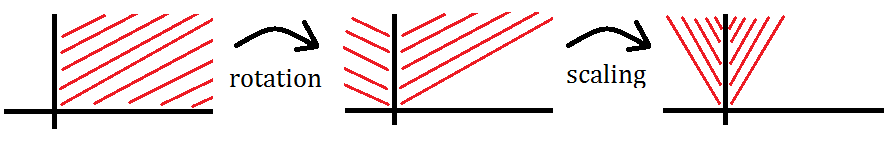
\includegraphics[scale=0.6]{images/Course7_equivalenceCones.png}\\
   \label{bruno}
  \caption{Solving a problem on one cone is equivalent to solve it on a newly obtained cone via rotation and scaling.}
\end{figure}
\end{center}

The conic optimization is useful since it is more general than linear optimization. The sets considered are not polyhedrons anymore but rather curved sets. Thus, it can cover more problems.

\subsection{Lorentz cone}
A common example of a cone is the Lorentz cone or ice cream cone. It is defined such as: 
\[
\mathbb{L}^n = \{(x_0,\dots, x_n) \in \mathbb{R}^{n+1} \mid \sqrt{x_1^2+...+x_n^2} \le x_0 \}
\]

One can verify it is indeed a cone by checking that when multiplying a value in the cone by a scalar it stays in the cone; and that addition is preserved (intuition: rule of parallelogram). Also, checking if the hull is a cone is the same as checking whether it is convex or not.

\begin{example}
\begin{leftbar}
Let the problem:
\begin{center}
$\max (y_1+y_2)$ \\
$y_1^2+y_2^2 \leq 7$
\end{center}

One notes that the constraint is quadratic and semi-definite positive. One would like to formulate the problem as linear, except for the cone. All that is non-linear shall be put in the cone, hence: 

\begin{align*}
y_1^2+y_2^2 \leq 7 \, 
\Leftrightarrow \, 
\sqrt{y_1^2+y_2^2} \leq \sqrt{7} \\ \vspace{0.5cm}
\Updownarrow \\ \vspace{0.5cm}
\left( \begin{array}{c}
\sqrt7 \\
y1\\
y2 \end{array} \right) 
\in \mathbb{L}^2 \
\Leftrightarrow \, 
\
\left( \begin{array}{c}
\sqrt7 \\
y1\\
y2 \end{array} \right) 
\succeq_{ \mathbb{L}^2}
\left( \begin{array}{c}
0\\
0\\
0\\\end{array} \right) \\ \vspace{0.5cm}
\Updownarrow \\ \vspace{0.5cm}
\left( \begin{array}{c}
\sqrt7 \\
0\\
0 \end{array} \right) 
\succeq_{ \mathbb{L}^2}
\left( \begin{array}{c}
0 \\
-y_1\\
-y_2 \end{array} \right) 
\end{align*} 

Finally:

\begin{center}
\[
C =\sqrt7, 
\hspace{1cm}
A = \left( \begin{array}{cc}
-1 & 0 \\
0 & -1 \end{array} \right), 
\hspace{1cm}
y = \left( \begin{array}{c}
y_1 \\
y_2 \end{array} \right)
\]
\end{center}
And the problem can be written as: 
\begin{center}
$\max (y_1+y_2)$ \\
$-y_1-y_2 \preceq_{\mathbb{L}^2} \sqrt7$
\end{center}
\end{leftbar}
\end{example}

\subsection{Requirements for $K$} 
\begin{enumerate}
\item $x \succeq 0$ and $x \preceq 0 \Rightarrow x = 0$

which means $K \cap (-K) = \{ 0 \}$ (the cone is \emph{pointed})

\item We define the strict inequality by $a \succ 0
\Leftrightarrow a \in int ~K$ (and $a \succ b$ iff $a-b \in int~
K$)

Hence we require $int~ K \neq \emptyset$ (the cone is
\emph{solid})

\item Finally, we would like to be able to take limits:
\[ \text{If } \{ x_i \}_{i \to \infty} \text{ with } x_i \succeq_K
0 \ \forall i,\ \text{then} \lim_{i \to \infty} x_i = \bar{x}
\Rightarrow \bar{x} \succeq_K 0 \] which is equivalent to saying
that $K$ is \emph{closed}. \end{enumerate} 


A convex cone $K$ that is solid, pointed and closed will be called a \emph{proper cone}.\\

As seen in section \ref{solving_diff_cones}, in the conic optimization theory, all the cones can always be merged as an only one according to the following definition.\\

\begin{definition} 
Considering several conic constraints \[ A_1^T y \preceq_{K_1} c_1
\text{ and } A_2^T y \preceq_{K_2} c_2 \] which are equivalent to
\[ c_1 - A_1^T y \in K_1 \text{ and } c_2 - A_2^T y \in K_2 \] one
introduces the product cone $K = K_1 \times K_2$ to write
\[ (c_1 - A_1^T y, c_2 - A_2^T y) \in K_1 \times K_2
\] \[ \Leftrightarrow \begin{pmatrix} c_1 \\ c_2
\end{pmatrix} -
\begin{pmatrix} A_1^T \\ A_2^T \end{pmatrix} \in K_1 \times K_2
\Leftrightarrow
 \begin{pmatrix} c_1 \\ c_2 \end{pmatrix} -
\begin{pmatrix} A_1^T \\ A_2^T \end{pmatrix} \succeq_{K_1 \times K_2} 0 \]
If $K_1$ and $K_2$ are proper, $K_1 \times K_2$ is also proper.
\end{definition}

However, in this course, and for the exercises, we will not merge the cones.

\subsection{Equivalence with convex optimization} 
Since a cone is convex, conic optimization can be related to convex optimization: conic optimization is clearly a special case of convex optimization. What about the reverse statement ?

\[ \min_{x \in \mathbb{R}^n} f(x) \text{ such that } x \in X \subseteq
\mathbb{R}^n \]

\begin{itemize}
\item The objective of a convex problem can be assumed
\emph{w.l.o.g.}\footnote{without loss of generality} to be \emph{linear}: $f(x) = c^T x$

\item The feasible region of a convex problem can be assumed
\emph{w.l.o.g.} to be in the \emph{conic} standard format: \[ X
= \{ x \in K \text{ and } A x = b \} \]
\end{itemize}

$\Rightarrow$ conic optimization \emph{equivalent} to convex
optimization. \\

One can prove that everything in the use of conic optimization, must be convex. Considering the conic constraint: 
\begin{equation}
c-A^Ty \in K \nonumber 
\end{equation}
choosing $K$ to be convex is a good way to ensure the constraint to be convex too since linear transformations preserve convexity. \\

\section{Duality}
What about the conic dual problems ? Since we generalized
\[ \max b^T y \text{ s.t. } A^T y \leq c \] to
\[ \max b^T y \text{ s.t. } A^T y \preceq_K c \] it could be tempting to generalize
\[ \min c^T x \text{ s.t. } Ax = b \text{ and } x \geq 0 \]
to
\[ \min c^T x \text{ s.t. } Ax = b \text{ and } x \succeq_K 0 .\]
However, this is not the right primal-dual pair ! Actually, we must also dualize the cone; and the corresponding correct primal-dual pair is given by 
\vspace{0.3cm} \[ \max b^T y \text{ such that } A^T y \preceq_K c \]
\[ \min c^T x \text{ such that } Ax = b \text{ and } x \succeq_{K^*} 0 \]

\vspace{0.3cm}
where we introduce the dual cone $K^*$ defined as 
\[ K^* = \{ z \in \mathbb{R}^n \text{ such that }
x^T z \geq 0 \ \forall x \in K \} \]

\begin{itemize}
\item $K^*$ is a convex cone, called the \emph{dual} cone of $K$;
\item $K^*$ is always \emph{closed}, and if $K$ is closed, $(K^*)^* = K$; \item $K$ is \emph{pointed} (resp. 
   solid) $\Rightarrow K^*$ is \emph{solid} (resp. pointed) \item Cartesian products: $(K_1 \times K_2)^*
   = K_1^* \times K_2^*$;
\item $(\mathbb{R}^n+)^* = \mathbb{R}^n+, (\mathbb{L}^n)^* = \mathbb{L}^n, (\mathbb{S}_+^n)^* = \mathbb{S}_+^n$: these cones are self-dual, but there are (many) cones which are not.
\end{itemize}


% \end{document}
	

%\documentclass[11pt,a4paper]{article}
%\usepackage[utf8]{inputenc}
%\usepackage[francais,english]{babel}
%\usepackage[T1]{fontenc}
%\usepackage{amsmath}
%\usepackage{amsfonts}
%\usepackage{graphicx}
%\usepackage{amssymb}
%\usepackage{fullpage}
%\usepackage{fancybox}
%\usepackage[Lenny]{fncychap}
%\usepackage{gensymb}
%\usepackage{color}
%\usepackage{array}
%\usepackage{url}
%\usepackage{here}
%\usepackage[final]{pdfpages}
%\usepackage{wrapfig}
%\usepackage[version=3]{mhchem}
%\usepackage{numprint}
%\usepackage[toc,page]{appendix}
%\usepackage{bibentry}
%\usepackage{eurosym}
%\usepackage{lmodern}
%\usepackage{subfig}
%\usepackage{listings}
%\usepackage{color}
%\usepackage{textcomp}
%\definecolor{listinggray}{gray}{0.9}
%\definecolor{lbcolor}{rgb}{0.9,0.9,0.9}
%\usepackage{numprint}
%\usepackage[toc,page]{appendix}
%\usepackage{booktabs}
%\usepackage{bm}
%\usepackage{amssymb}
%
%
%
%\title{LINMA2471 : Optimization models and methods: Lecture 8}
%\author{Antoine Noé, Ad'Oul Ismail, Dehem Boris}
%\date{S10 - November, 18th 2015}
%
%\begin{document}
%\maketitle


\subsection{Exercise sessions on conic optimization}

In chapter \ref{Ch1}, we saw how to model convex problems. In chapter \ref{Ch2}, we studied methods that deal with that type of problems. The disadvantage of those methods is that they can be quite slow, especially when compared with linear solvers (for linear systems). We now look at a certain class of convex problems, conic problems, that conserve some of the properties that make linear systems so effective. In particular, we want our problems to have duality, because a dual problem will be a much better problem to certify optimality. We start by looking at quadratic functions $x^TQx$ \\

\noindent $x^Tx$\\
$\downarrow$ \qquad $Q \geq 0 \Longleftrightarrow Q=LL^T$ \\
$x^TQ$ \\
$\Updownarrow$ \\
$(L^tx)^T(L^Tx)$\\

This last expression $(L^tx)^T(L^Tx)$ is a linear transformation of $x^Tx$ so it preserves convexity.\\

In this section, we will do a quick reminder on some exercises of \textcolor{red}{Exercise session 5} on conic modelling: second order cone and duality. 

\subsubsection{Exercise 2}
In this exercise, we have a rotated second order cone $\mathbb{L}^n_R $
$$\mathbb{L}^n_R=\{(x,y,z)\in \mathbb{R}^n\times \mathbb{R}_+ \times \mathbb{R}_+ \mid x_1^2+x_2^2+...+x_n^2 \leq yz \}$$ 
We can prove that this set is a cone by replacing it by a second order cone. Why do we then use the rotated second order cone? The rotated second order cone is usefull because it makes some models easier (for example, the models in exercise 3). 

\subsubsection{Exercise 4}
The question here is "how do we deal with conic modelling of \textbf{functions}"? Let's take example (d). \\
Function $(x,z)\rightarrow \dfrac{\parallel x \parallel^2}{z}$ (on the domain $z>0$). We have $$\underset{\underset{z\in \mathbb{R}>0}{x\in \mathbb{R}^n}}\min \dfrac{\parallel x \parallel^2}{z}$$
This is not a conic problem because there is no linear objective. Our goal is to transform it in order to have a linear objective:
$$\underset{\underset{z\in \mathbb{R}>0}{x\in \mathbb{R}^n}}\min \dfrac{\parallel x \parallel^2}{z}$$
$$\Updownarrow$$
$$\underset{\underset{z\in \mathbb{R}>0}{x\in \mathbb{R}^n}}{\underset{t\in\mathbb{R}}\min}\ t\qquad s.t.$$
$$\parallel x \parallel^2 \leq tz$$
Now, we have a linear objective, and constraints of the rotated second order cone type.

\subsubsection{Exercise 6 : Conic duality}
In this exercise, we need to find the dual for some optimization problems, using an equivalent conic formulation. To compute a dual problem, we need to reformulate it to a standard conic formulation.\\
Let's consider the dual and the primal problem: 
$$(D)\qquad \qquad \max \, b^Ty \qquad \longleftrightarrow \qquad \min \, c^Tx \qquad \qquad (P)$$ 
$$ \qquad A^Ty \preceq_K c \qquad \qquad \qquad Ax=b$$
$$ \qquad \qquad \qquad \qquad \qquad \qquad \quad x\succeq_{K^*}0$$
where (D) stands for the dual problem and (P) the primal problem. 
Note that for the positive real axis, second order cones and the semi definite cone: $K=K^*$.

\subsection{Example of duality}

\subsubsection{Primal problem}
Let's consider the following problem: 
\begin{align*}
&\min \, \sqrt{z^TQz} \qquad (Q\geq 0)\\
&Cz \leq d
\end{align*}

The function we minimize is quadratic, and Q is positive semi-definite. The constraint $Cz \leq d$ is a linear constraint. We need to transform this formulation into one of the two formulations above. \\
Let's say we first want to take care of the objective (since it is quadratic). 
$$\min \, t$$
$$\qquad \qquad \qquad \qquad \sqrt{z^TQz}\leq t \qquad \qquad Q=LL^T$$
$$\parallel L^Tz \parallel \leq t$$
This is equivalent 
$$\begin{pmatrix}
t\\
L^Tz
\end{pmatrix} \in \mathbb{L}^n$$

Now, we want to reformulate the linear constraint: 
$$Cz\leq d \Longleftrightarrow d-Cz \geq 0$$
This can be written as 
$$d-Cz \in \mathbb{R}^m_+$$
Now, we are going to write everything using the cones: \\
Let $y=\begin{pmatrix}
t\\
z
\end{pmatrix} \in \mathbb{R}^{n+1}$ (t is composed of 1 element and z of n elements). \\
Objective $-\max \, b^Ty$ with $b=\begin{pmatrix}
-1\\
0\\
. \\
. \\
. \\
0
\end{pmatrix}$\\
Constraint: $c-A^Tu \geq_K 0 $ with $K= \mathbb{R}^m_+ \times \mathbb{L}^n$ (big vector with the top part being $\mathbb{R}^m_+$ and the bottom part $\mathbb{L}^n$)\\

$\begin{bmatrix}
d-Cz\\
\_ \_ \_ \_ \_ \\
t\\
L^Tz
\end{bmatrix} \in K$, where $d-Cz \in \mathbb{R}^m_+$ and $\begin{bmatrix}
t\\
L^Tz
\end{bmatrix} \in \mathbb{L}^n$\\
Note that $d-Cz$ is composed of m elements, t of one element and $L^Tz$ of n elements. \\

We are not completely done yet because we still need $c$ and $A^T$:\\
$$c = \begin{pmatrix}
d\\
\_ \_ \_ \\
0\\
. \\
. \\
. \\
0
\end{pmatrix} \qquad A^T= \begin{pmatrix}
0 & C\\
-1 & 0^{1\times n}\\
0^{n\times 1} & -L^T
\end{pmatrix}
$$
The first column of $A^T$ corresponds to the coefficients of t. \\

By telling our solver the different matrices and the cone, it will solve the problem. Why is this useful? Because now we can write the dual without a problem.

\subsubsection{Dual Problem}
$$K^*= (\mathbb{R}^m_+ \times \mathbb{L}^n)^*= (\mathbb{R}^m_+)^* \times (\mathbb{L}^n)^*= \mathbb{R}^m_+ \times \mathbb{L}^n = K$$
Let's consider $x= \begin{pmatrix}
u \\
v
\end{pmatrix} $ with $u \in \mathbb{R}^m_+$ and $v \in \mathbb{L}^n$\\
The dual is 
$$-\min \, \begin{bmatrix}
d \\
0
\end{bmatrix}^T \begin{pmatrix}
u\\
v
\end{pmatrix} $$

\begin{equation}
\begin{bmatrix}
0^{1\times n} & -1 & 0^{1\times m}\\
C^T & 0^{k\times 1} & -L
\end{bmatrix}\begin{pmatrix}
u\\
v
\end{pmatrix}=
\begin{pmatrix}
-1\\
0^{k\times 1}
\end{pmatrix}
\end{equation}
Where n, m and k are the dimensions of $C$ and $L$.
 
 After simplifying, we have \\
 $$-\min \, d^Tu$$
 $$u \geq 0$$
 $$v_0 \geq \parallel (v_1 ... v_n) \parallel$$
 $$C^Tu - L\begin{pmatrix}
 v1\\ 
 .\\
 .\\
 .\\
 v_n
 \end{pmatrix} = 0 $$
 $$-v_0=-1$$
 
 By putting $w=(v_1 ... v_n)$, we get the following simplified model 
$$-\min \, d^Tu$$
$$u \geq 0$$
$$\parallel w \parallel \leq 1$$
$$C^Tu = Lw$$
This model cannot be simplified any further.


\subsection{Theorems and properties of Dual}
After this example of conic dual computation, we want to study the properties of the conic dual optimization and some of its theorems. One interesting design allows to prove some theorems. Let us first explain this design to eventually find the dual of the primal conic problem (P):
\begin{align*}
\min&\textbf{b}^T\textbf{y}\\
             &\textbf{A}^T\textbf{y}\preceq_K \textbf{c}
\end{align*}

First, to build the standard dual problem, we write the constraints as a system of inequations where coefficients $\lambda_i \geq 0$ multiplies $c_i$ (positivity of $\boldsymbol{\lambda}$ assures the preservation of inequalities):
\[\begin{bmatrix}
 a_1^T \boldsymbol{y} \leq c_1\\
 a_2^T \boldsymbol{y} \leq c_2\\
 \vdots\\
 a_n^T \boldsymbol{y} \leq c_n
\end{bmatrix}
\begin{matrix}
 \times \lambda_1\\
 \times \lambda_2\\
 \vdots\\
 \times \lambda_n
\end{matrix}
\over
(\sum_{i=1}^{n}\lambda_i a_i)^T \leq \sum_{i=1}^{n}\lambda_i c_i\]

We can write the new system system as:
\[(\boldsymbol{A}\boldsymbol{\lambda})^T \boldsymbol{y} \leq \boldsymbol{c}^T \boldsymbol{\lambda}
\]
The dual goal is to find the best upper bound for this system. This is, that best upper bound is found by minimizing the dual objective.\\

When $\boldsymbol{A\lambda}=\boldsymbol{b}$, we get the system $\boldsymbol{b}^T \boldsymbol{y} \leq \boldsymbol{c}^T \boldsymbol{\lambda}$. The upper bound depends on $\boldsymbol{\lambda}$ and the dual problem (D) becomes:

\begin{eqnarray*}
\min & & \boldsymbol{c}^T \boldsymbol{\lambda}\\
\text{such that}& &\boldsymbol{A\lambda}=\boldsymbol{b}\\
             & &\boldsymbol{\lambda} \geq \boldsymbol{0}
\end{eqnarray*}

In a conic problem, we have:
\[\begin{bmatrix}
 a_1^T \boldsymbol{y}\\
 a_2^T \boldsymbol{y}\\
 \vdots\\
 a_n^T \boldsymbol{y}
\end{bmatrix} \preceq_K \begin{bmatrix}
 c_1\\
 c_2\\
 \vdots\\
 c_n
\end{bmatrix}\]

A simple example on the Lorentz cone show that the standard dual does not always work in conic optimization: let us have:
\[\begin{bmatrix}
 0\\
 0\\
 0
\end{bmatrix} \preceq_{\mathbb{L}^2} \begin{bmatrix}
 1\\
 -1\\
 0
\end{bmatrix}\]
This is valid since on the Lorentz cone we must have in this case the condition $1\geq ||(-1,0)||$ satisfied, which is the case. However, if we now multiply $\boldsymbol{c}^T$ by a positive vector $\boldsymbol{\lambda}=(2,10,0)$, we get then:
\[\begin{bmatrix}
 0\\
 0\\
 0
\end{bmatrix} \preceq_{\mathbb{L}^2} \begin{bmatrix}
 1\\
 -1\\
 0
\end{bmatrix}\begin{matrix}
 \times 2\\
 \times 10\\
 \times 0
\end{matrix}\over
0 \stackrel{?}{\leq} 2-10+0\]
In this example, the positivity of $\boldsymbol{\lambda}$ does not preserve the inequalities as we need to in order to use the standard dual formulation.\\

\subsubsection{Necessary and sufficient condition}
The idea is that when starting with something positive and multiplying by $\boldsymbol{\lambda}$, we must stay positive. For instance a good multiplier on the Lorentz cone would be such that:
\[\begin{bmatrix}
 0\\
 0\\
 \vdots\\
 0
\end{bmatrix} \preceq_{\mathbb{L}^2} \begin{bmatrix}
x_1\\
x_2\\
\vdots\\
x_n
\end{bmatrix}\begin{matrix}
 \times \lambda_1\\
 \times \lambda_2\\
 \vdots\\
 \times \lambda_n
\end{matrix}\over
0 \leq \sum_{i=1}^{n}\lambda_ix_i\]

The condition to have a correct $\boldsymbol{\lambda}$ is the following: whatever the $\boldsymbol{x}$ we start with, $\boldsymbol{\lambda} \in K^*$ if $\boldsymbol{\lambda}^T\boldsymbol{x} \geq 0$:
\[\boldsymbol{\lambda}^T\boldsymbol{x}\geq 0 \textrm{  } \forall \boldsymbol{x} \in K \Leftrightarrow \boldsymbol{\lambda} \in K^* \]
Where $K^*$ is the dual cone.

\begin{example}
\begin{leftbar}
\textbf{Dual cone for $\mathbb{R}_+$ and $\mathbb{R}_+^n$}\\

$\Rightarrow(\mathbb{R}_+)^*=?$\\
$(\mathbb{R}_+)^*=\{\lambda | x \lambda \geq 0\textrm{, } \forall x \in \mathbb{R}_+ \}$
\begin{itemize}
\item $\lambda \geq 0$ : this works because $\lambda x \geq 0$ when $x,\lambda \geq 0$
\item $\lambda < 0$ : one can pick $x=1$ and observe that $x \lambda<0$, that is $\lambda \notin (\mathbb{R}_+)^*$
\end{itemize}

$\Rightarrow(\mathbb{R}_{+}^n)^*=?$\\
$(\mathbb{R}^n_+)^*=\{\boldsymbol{\lambda} | \boldsymbol{x}^T \boldsymbol{\lambda} \geq 0\textrm{, } \forall \boldsymbol{x} \in \mathbb{R}^n_+ \}$
\begin{itemize}
\item $\boldsymbol{\lambda} \geq 0$ : this works because $\boldsymbol{x}^T \boldsymbol{\lambda} \geq 0$ when $\boldsymbol{x},\boldsymbol{\lambda} \geq 0$
\item $\lambda_i < 0$ : one can pick a $\boldsymbol{x}$ such that one of its elements is negative, but not negative everywhere: 
\[\boldsymbol{\lambda}=\begin{bmatrix}
 ?\\
 \vdots\\
 <0\\
 \vdots\\
 ?
\end{bmatrix},\boldsymbol{x}=\begin{bmatrix}
 0\\
 \vdots\\
 1\\
 \vdots\\
 0
\end{bmatrix}\]
This way, $\lambda_i^T x_i < 0$, and that implies dual cone is $(\mathbb{R}_{+}^n)$.
\end{itemize}

\end{leftbar}
\end{example}

\begin{example}
\begin{leftbar} 
\textbf{Dual cone for $\mathbb{L}^n$}

$\Rightarrow(\mathbb{L}^n)^*=?$\\
$(\mathbb{L}^n)^*=\{\lambda | x^T \lambda \geq 0\textrm{, } \forall x \in \mathbb{L}^n \}$
\begin{itemize}
\item $\lambda \in \mathbb{L}^n$ : $x^T\lambda = x_0\lambda_0 + [x_1 ... x_n][\lambda_1 ... \lambda_n]^T$:\\
Because we know= $x_0\geq ||x_1...x_n||$ and $\lambda_0 \geq ||\lambda_1...\lambda_n||$, we can say: \begin{align*}
x^T\lambda &\leq x_0\lambda_0+||x_1...x_n||||x_1...x_n||\\
&\geq x_0\lambda_0-||x_1...x_n||||x_1...x_n|| \geq 0
\end{align*}
\item $\lambda \notin \mathbb{L}^n$: $\lambda_0 < ||\lambda_1 ..  \lambda_n||$ \\
One can pick $x$ the following way: $x_0 = ||\lambda_1...\lambda_n||$; $[x_1..x_n] = -[\lambda_1 ... \lambda_n]$\\
In that case, \begin{align*}
x^T\lambda &= \lambda_0||\lambda_1 ..  \lambda_n|| - ||\lambda_1 ..  \lambda_n||^2\\
&= (\lambda_0 - ||\lambda_1 ..  \lambda_n||)||\lambda_1 ..  \lambda_n||<0
\end{align*}
\end{itemize}
This implies the second order cone is self-dual.

\end{leftbar}
\end{example}

\subsubsection{Theorems}
We can conclude what has been done with two theorems on conic duality:

\begin{theorem}[Weak duality]
If x is feasible for the primal (P) and y is feasible for the dual (D), then $$c^Tx\ge b^Ty$$
\end{theorem}

\begin{theorem}
Under some assumptions, optimal value of (P) is equal to the optimal value of (D).
\end{theorem}




%\end{document}
	

%\documentclass[12pt,a4paper]{article}
%
%\usepackage[utf8]{inputenc}			            % accents en francais
%\usepackage[T1]{fontenc}			            % accents et cesure
%\usepackage{lmodern}				            % image vectorielle
%\usepackage{graphicx}                           % image stylees
%\usepackage{epstopdf}
%\usepackage{url}
%\usepackage{array}                              % faire des beaux tableaux
%\usepackage{amsmath,amsfonts,amssymb,amsthm}    % faire des maths
%\usepackage{mathtools}                          % contient asmath mais pas amsfonts et amssymb
%\usepackage{empheq}                             % encadrer equations
%\usepackage{enumerate}				            % listes avec (a), (b)
%\usepackage{geometry}                           % changer les marges
%\usepackage{xcolor}
%\usepackage{colortbl}
%\usepackage{multicol}
%\usepackage{sectsty}                            % titre colores
%\usepackage{lipsum}                             % lipsum[1-5]
%\usepackage{hyperref}
%\usepackage{caption}                            % modifier legendes
%\usepackage{listings}
%\usepackage{slashbox}
%\usepackage[french]{babel}
%
%\geometry{left=25mm,right=25mm,top=15mm,bottom=20mm}
%
%\theoremstyle{definition}
%\newtheorem{mydef}{Definition}
%
%\theoremstyle{plain}
%\newtheorem{mythm}{Theorem}
%
%\captionsetup{labelsep=endash,margin=20mm}
%\captionsetup{font={sf},labelfont={sc,small},textfont={small}}
%
%\DeclareMathOperator{\reals}{\mathbb{R}}
%\DeclareMathOperator{\suchthat}{\;\;\;\;\boxed{\text{s.t.}}\;\;\;\;}
%
%\title{LINMA2471: Optimization models and methods \\\smallskip --- Lecture 9 (Conic Modelling III) ---}
%\author{Berger Guillaume, Fabri Arnaud, Hamaide Valentin}
%\date{S11 - November, 25th 2015}
%
%\begin{document}
%\maketitle


%In this third lecture about conic modelling we will interest ourselves at applications of dual problem, mainly application in sensitivity analysis and robust optimisation. Then we will have a short look at optimisation with positive semi-definite matrices.

%%%%%%%%%%%%%%%%%%%%%%%%%%%%%%%%%%%%%%%%%%%%%%%%%%%%%%%%
\subsection{Strong duality for conic optimisation problems}

The primal-dual formulation of a conic optimisation problem has already been covered in the precedent lecture notes. They also showed how we come to the weak duality theorem and the need to work with the dual cone. Let us recall the primal-dual formulation:
\begin{eqnarray*}
    \text{(PRIMAL)} & & \text{(DUAL)} \\
    \min_{x\in \mathbb{R}^n} c^T x & \longleftrightarrow & \max_{y\in\mathbb{R}^m} b^Ty \\
    Ax = b & & A^Ty \preceq_K c\\
		x \succeq_{K^*} 0 & & 
\end{eqnarray*}

The weak duality theorem states that if $x$ is an admissible solution of the primal and $y$ is an admissible solution of the dual then we must have that $c^Tx\geq b^Ty$. First of all this show that if for example the dual is (upper)-unbounded then the primal is infeasible. Reversely, if the primal is (lower)-unbounded then the dual is infeasible.

Imagine a algorithm has converged to a feasible solution $y$ of the dual. And it want to know if the solution is optimal or not. If it has also a solution $x$ of the primal and that $c^Tx=b^Ty$ then $y$ and $x$ are the optimum $y^*$ and $x^*$ of the dual and primal respectively.

We can wonder if we always have $c^Tx^* = b^Ty^*$. On the same way, if the primal is infeasible, does it always mean that the dual is unbounded? To answer both questions, let us consider the conic problem with the following parameters:
\begin{eqnarray*}
 A = \left[\begin{array}{ccc} -1 & 0 & -1 \\ 0 & -1 & 0 \end{array}\right] ,
b = \left[\begin{array}{c} 0 \\ -1 \end{array}\right] ,
c = \left[\begin{array}{c} 0 \\ 0 \\ 0 \end{array}\right] ,
K = K^* = \mathbb{L}^2
\end{eqnarray*}
Any admissible solution of $Ax=b$ is of the form $x=(k,1,-k)$ so that $x\notin \mathbb{L}^2$. Thus the primal is infeasible. But the dual has only one admissible solution $y=(0,0)$ which is thus the optimal solution and the dual objective is bounded.

Another example involves the cone $\mathbb{S}^n_+$ of symmetric positive semi-definite matrices of order $n$. We will discuss this cone further in the following chapter. The primal formulation of this example is:
\begin{eqnarray*}
\min_{x\in\mathbb{R}^6} & & (kx_3 - 2x_4)  \\
\text{such that} & & \left[\begin{array}{ccc} x_1 & x_4 & x_5 \\ x_4 & x_2 & x_6 \\ x_5 & x_6 & x_3 \end{array}\right] \in \mathbb{S}^3_+ \\
 & & \left[\begin{array}{c} x_3 + x_4 \\ x_2 \end{array}\right] = \left[\begin{array}{c} 1 \\ 0 \end{array}\right]
\end{eqnarray*}
If you are motivated, we can show that the optimal solution is such that $c^Tx^* = k$. We are not yet able to write the dual of this problem but we will spoil that the optimal dual cost is $b^Ty^* = 2$. Thus we have a non-zero duality gap. The duality gap is defined to be the non-negative quantity $c^Tx^* - b^Ty^*$.

Last but not least, a third example involving semi-definite cones:
\begin{eqnarray*}
 \min_{x\in\mathbb{R}^3} & & x_1 \\
 \text{such that} & & \left[\begin{array}{cc} x_1 & x_3 \\ x_3 & x_2 \end{array}\right] \in \mathbb{S}^2_+ \\
& & x_3 = 1 
\end{eqnarray*}
The eigenvalues of the matrix are such that $\lambda_1 + \lambda_2 = x_1 + x_2$ and $\lambda_1\lambda_2 = x_1x_2 - 1$. They must be non-negative, so that we find that $x_1>0$. There is thus no minimum, only an infimum when $x_1$ tends to be zero.

In each one of the previous examples, we can identify the same cause of our troubles: the affine subspace defined by the linear constraint (of the primal problem) is tangent to the cone. The interior of the admissible primal domain is thus empty. This observation leads us to the strong duality theorem. But first, let us introduce a new definition.

\begin{definition}
A feasible solution to a conic (primal or dual) problem is strictly feasible if and only if it belongs to the interior of the cone. For the primal, we must have $Ax=b$ and $x \succ_{K^*} 0$. And for the dual, $y$ must satisfy $A^Ty \prec c$.
\end{definition}

\begin{theorem}[Strong duality]
If the dual problem admits a strictly feasible solution and is unbounded, then the primal is infeasible. If the dual problem admits a strictly feasible solution and is bounded, then the primal is feasible and $c^Tx^*=b^Ty^*$. The reverse proposition holds for the primal.
\end{theorem}

\begin{table}
\centering
\begin{tabular}{|l||c|c|c|}
    \hline
    \backslashbox{Dual}{Primal} & Unbounded & Finite & Infeasible \\ \hline\hline
    Unbounded & KO & KO & OK \\ \hline
    Finite & KO & $c^Tx_*\geq b^Ty_*$ & OK \\ \hline
    Infeasible & OK & OK & OK \\ \hline
\end{tabular}
\caption{Recapitulate of the weak duality theorem. The theorem is always true but does not tell a lot of things.}
\label{tab_weak}
\end{table}

\begin{table}
\centering
\begin{tabular}{|l||c|c|c|}
    \hline
    \backslashbox{Dual}{Primal} & Unbounded & Finite & Infeasible \\ \hline\hline
    Unbounded & KO & KO & OK \\ \hline
    Finite & KO & $c^Tx_*=b^Ty_*$ & KO \\ \hline
    Infeasible & OK & KO & OK \\ \hline
\end{tabular}
\caption{Recapitulate of the weak duality theorem. The theorem can be used if either the dual or the primal has one strictly feasible solution.}
\label{tab_strong}
\end{table}

Before going on to the following section, let us formulate a little remark about the dual of a cone. Actually finding the dual of a cone is not always an easy task. This becomes really tedious if it must be done by a computer. This is the reason why most of the conic solvers work only with self-dual cones. The most used self-dual cones are: the first-order cone $\mathbb{R}^n_+$, the Lorentz cone $\mathbb{L}^n$ and the semi-definite cone $\mathbb{S}^n_+$.


%%%%%%%%%%%%%%%%%%%%%%%%%%%%%
\section{Robust optimisation}

In all the conic problems we have encountered before, the number of conic constraints was finite and thus the resulting cones was computable since it was the Cartesian product of a finite number of cones. Now consider the following example with a infinite number of linear constraints and $X$ a convex domain:
\begin{eqnarray*}
\min_{x\in X} & c^Tx\\
\text{such that}  & a^Tx \leq b & \forall a\in A
\end{eqnarray*}
We can satisfy all of the constraints by imposing:
$$ \left[\max_{a \in A} a^Tx \right] \leq b $$
This is not much better since we need to solve another optimisation problem in our original problem, but if we replace the last problem by his dual, we obtain:
\begin{eqnarray*}
\min_{x\in X} & & c^Tx\\
\text{such that} & & \left[\min_{\lambda \in L(x)} d^Tx \right] \leq b 
\end{eqnarray*}
The new cost vector $d$ depends on the set $A$. We can finally simplify this problem in:
\begin{eqnarray*}
\min_{x,\lambda} & & c^Tx \\
\text{such that}  & & d^Tx \leq b \\
& & x\in X \\
& & \lambda\in L(x)
\end{eqnarray*}

The way we can obtain the vector $d$ and the space $L(x)$ may seem a bit fuzzy at this point. To have a better view of the problem, consider the following example:
\begin{eqnarray*}
\min_{x\in X} & c^Tx\\
\text{such that} &  a^Tx \leq b & \forall a\in \mathrm{B}_2[a_0,r] \subset \mathbb{R}^n
\end{eqnarray*}
Thus each $a$ has the form $a_0 + rv$ where $\|v\|_2 \leq 1$. We can re-write the linear condition:
\begin{eqnarray*}
& (a_0^Tx - b) + rv^Tx \leq 0 & \forall v\in \mathrm{B}_2[0,1] 
\end{eqnarray*}
We use the Lorentz cone $\mathbb{L}^n \subset \mathbb{R}^{n+1}$ to formulate a conic problem:
\begin{equation*}
\left[ \begin{array}{rcl}
\max\limits_{t,v} & & (a_0^Tx - b)t + rv^Tx \\
\text{such that}& &  (t,v)\in \mathbb{L}^n 
\end{array}
\right] \leq 0
\end{equation*}
The dual of the problem is given by:
\begin{equation*}
\left[ \begin{array}{rcl} 
\min\limits_{\lambda} & & 0 \\
\text{such that} & & \lambda = (a_0^Tx - b,rx)\\
& &  \lambda\in \mathbb{L}^n 
\end{array}
 \right] \leq 0
\end{equation*}
And thus the original robust problem becomes a simple conic problem:
\begin{eqnarray*}
\min_{x\in X} & & c^Tx \\
\text{such that} & &  (a_0^Tx - b,rx) \in \mathbb{L}^n \subset \mathbb{R}^{n+1}
\end{eqnarray*}


%%%%%%%%%%%%%%%%%%%%%%%%%%%%%%%%%%%%
\section{Semi-definite optimisation}

We will now speak a bit further about the semi-definite cone. If we note $\mathbb{S}^n$ the set of symmetric matrices of order $n$, then the semi-definite cone is defined by:
\begin{equation*}
\mathbb{S}^n_+ = \left\lbrace X \in \mathbb{S}^n  \big|  v^TXv \geq 0 \hspace{5mm} \forall v\in \mathbb{R}^n \right\rbrace
\end{equation*}

Over the set $\mathbb{S}^n$, we defined the inner-product $\langle X,Y \rangle = \mathrm{trace}[X^TY]$. The dual $(\mathbb{S}^n_+)^*$ of the cone $\mathbb{S}^n_+$ is thus the set of $Y\in\mathbb{S}^n$ such that $\mathrm{trace}[X^TY]$ is non-negative for all $X\in\mathbb{S}^n_+$. We can show that $\mathbb{S}^n_+$ is auto-dual\footnote{For a simple proof, you can consult the lemma $12.5$ in \url{http://www.cs.cmu.edu/afs/cs.cmu.edu/academic/class/15859-f11/www/notes/lecture12.pdf}.}. The primal-dual formulation of a conic problem involving semi-definite constraints is given by:
\begin{equation*}
\begin{array}{ccc}
    \text{(PRIMAL)} & & \text{(DUAL)} \\
    \min\limits_{X\in\mathbb{S}^n} \langle C,X \rangle & \longleftrightarrow & \max\limits_{y\in\mathbb{R}^m}  b^Ty \\
    \langle A_i,X \rangle = b_i \hspace{5mm} \text{for} \hspace{5mm} i\in\lbrace 1,\dots,m\rbrace & & C -\sum\limits_{i=1}^m A_iy_i \in \mathbb{S}^n_+ \\
    X \in \mathbb{S}^n_+ & &
\end{array} \:.
\end{equation*}
%
%\end{document}
	

%\documentclass[a4paper]{article}
%
%\usepackage[english]{babel}
%\usepackage[utf8]{inputenc}
%\usepackage{amsmath}
%\usepackage{amssymb}
%\usepackage{graphicx}
%\usepackage[colorinlistoftodos]{todonotes}
%\usepackage[left=2cm,right=3cm,top=2cm,bottom=1.3cm]{geometry}
%
%
%\title{LINMA2471: Optimization models and methods: course 11}
%\author{BROGNIET Adrien, DEFOUR Loïc, NINANE Charles}
%\date{December 1, 2015}
%
%\begin{document}
%\maketitle


\section{Conic modeling}
So far we have seen two types of cones: 
\begin{itemize}
\item $\mathbb{R}_n^+$ first order cone to represent linear constraints.
\item $\mathbb{L}^n$ second order cone to represent quadratics constraints like ratio, second and third power, ...
\end{itemize}
Theses cover a large class of problems but we will see a third type of cone. 
\subsection{Positive semi-definite cone}
A positive semi-definite cone is defined as: \{ M $\in \mathbb{S}^n | M \succeq 0 $ \} where $ \mathbb{S}^n$ is the set of symmetric matrices of size n. 
The following definitions of a positive semi-definite matrix are equivalent:
\begin{itemize}
\item $\mathbb{M} \succeq 0 $
\item All eigenvalues of M are greater than 0.
\item $\exists B \in \mathbb{R}^{n \times r}: M = BB^T  $ (kind of Cholesky factorisation)
\item $\forall x: x^T M x \geq 0$  
\end{itemize}

\subsubsection{Example conic optimization with semi-definite cone}
Find a symmetric matrix M such that:
\begin{itemize}
\item $ M = \begin{pmatrix}
   1 & 2 & 5\\
   2 & x & -1\\
   5 & -1 & y
\end{pmatrix}$ 
\item $\lambda_{max}$ is minimum. 
\end{itemize}
$\emph{Idea:}$
$\newline$
Let $M \in \mathbb{S}^n$ with eigenvalues $\lambda_1, \cdots, \lambda_n$. The eigenvalues are real because M is symmetric. It's easy to see that $ M + \Delta I \in \mathbb{S}^n$ has eigenvalues $ \lambda_1 + \Delta, \cdots, \lambda_n + \Delta $. By applying a shift on the diagonal of M we also shift the eigenvalues. By applying these observations to matrix M we can write the following \textcolor{red}{some of the $\geq$ or $\succeq$ seem to be inverted}: 
All eigenvalues of M $\geq 0 \Leftrightarrow M \succeq  0 \Leftrightarrow \lambda_{min}(M) \geq 0$
$\newline$
All eigenvalues of M $\geq 1 \Leftrightarrow M - I \succeq 0 \Leftrightarrow \lambda_{min}(M) \geq 1$
$\newline$
All eigenvalues of M $\geq c \Leftrightarrow M - cI \preceq 0$  (linear even if c is a variable)$  \Leftrightarrow \lambda_{min}(M) \geq c$
$\newline$
All eigenvalues of M $\leq c \Leftrightarrow M - cI \preceq 0   \Leftrightarrow \lambda_{max}(M) \leq c \Leftrightarrow - (M-cI) \succeq 0 = cI-M \succeq 0$ which is also a linear constraint.
$\newline$
$\newline$
We can now reformulate the optimization problem as:

$$ \min_{x,y,t} t \textnormal{ s.t } - \begin{pmatrix}
   1 & 2 & 5\\
   2 & x & -1\\
   5 & -1 & y
\end{pmatrix} + tI \succeq 0 $$ 

\chapter{Interior-point methods}	

\section{Pros and cons (of the Newton's method)}
\vspace{0.3cm}
\begin{tabular}{l|l}
\multicolumn{1}{c|}{Pros} & \multicolumn{1}{c}{Cons} \\ 
\hline
 & \\
- Faster convergence than first order methods & - More expensive computation \\
 & \\
- Potential quadratic convergence under specific conditions & - Not always well defined \\
 & \\
 & -  Not globally convergent 
\end{tabular}

\section{Computing the Newton's method}
We consider the unconstrained optimization program :
$$ \underset{x}{\min} \hspace{0.1cm} f(x) $$
$$ x \in \mathbb{R}^n $$
We use the second order Taylor expansion to write :
$$ f(x) = f(x_k + h) \approx f(x_k) + \nabla f(x_k)^T h + \frac{1}{2} h^T\nabla^2 f(x_k) h$$
with $x_k$ a fixed point and h a step such that $x_k,h \in \mathbb{R}^n $. We know that the stationary points of the function $f$ are reached when $\frac{ \partial f(x_k+h)}{\partial h} = 0$. Regarding the previous approximation, we have :
$$\frac{ \partial f(x_k+h)}{\partial h} = \nabla f(x_k) + \nabla^2 f(x_k) h $$
Therefore we can choose the step $h$ such that it satisfies the linear system :
$$\nabla^2 f(x_k) h = -\nabla f(x_k) $$
Assuming $\nabla^2 f(x_k)$ is invertible, we have :
$$ h = -\nabla^2 f(x_k)^{-1} \nabla f(x_k)$$
The Newton's method is then:

\begin{lstlisting}[mathescape,caption=Newton Algorithm]
Given $x_0$, $f$, $\nabla f$, $\nabla^2 f$ invertible, $k=0$
Repeat
$x_{k+1} = x_k - \nabla^2 f(x_k)^{-1} \nabla f(x_k) $
$k \leftarrow k+1$
\end{lstlisting}

\begin{example}
\begin{leftbar} 
Using the Newton's method, we can find the global minimum of the function $f(x) = x^2$ in one iteration $ \Longrightarrow x^+ = x - (2)^{-1}(2x) = 0$.
\end{leftbar}
\end{example}

\begin{example}
\begin{leftbar} 
Let us apply the Newton's method on $f(x) = -\cos(x)$. \\
We get that $x^+ = x - (\cos(x))^{-1}(\sin(x)) = x - \tan(x) = x - (x + \mathcal{O}(x^3))$ (near to 0, quadratic convergence) 
\end{leftbar}
\end{example}

\begin{example}
\begin{leftbar} 
Let us apply the Newton's method on $f(x) = x^4$. \\
We get that $x^+ = x - (12x^2)^{-1}(4x^3) = x - \frac{x}{3} = \frac{2}{3}x$. \\
We have a linear convergence.  \\
Why is that ? $f(x)$ has a "flat" minimum $\Longrightarrow \mbox{ in } x^* = 0, \nabla^2f(x^*) = 12x^* = 0 \nsucc \mu$.
\end{leftbar}
\end{example}

\subsection{Conditions for quadratic convergence}
\begin{theorem}{(Quadratic convergence)}Let $f \in \mathcal{C}^2$. If $\nabla^2f$ is $M$-Lipschitz and $x^*$ is a minimum of $f$ such that $\nabla^2f(x^*) \succeq \mu I$ (with $\mu \in \mathbb{R}$ and $I$ the identity matrix), then for any $x$ such that $||x-x^*|| \leq \frac{\mu}{2M}$ we have :
$$ ||x^+-x^*|| \leq \frac{M}{\mu} ||x-x^*||^2 \hspace{0.3cm}$$
with $x^+ = x - \nabla^2 f(x)^{-1} \nabla f(x)$ well defined.
\end{theorem}

\begin{example}
\begin{leftbar}
$\frac{\mu}{2M} \longmapsto \frac{M}{\mu} \cdot \left(\frac{\mu}{2M}\right)^2 = \frac{\mu}{4M} \longmapsto \frac{M}{\mu} \cdot \left(\frac{\mu}{4M}\right)^2 = \frac{\mu}{16M}$ (quadratic convergence) \\
After $k$ steps, we get $\frac{\mu}{M} \cdot \frac{1}{2^{2^{k-1}}}$.
\end{leftbar}
\end{example}

\subsection{Change of variables}
We have seen that an iteration of the Newton's method is defined by $x \longmapsto x - \nabla^2f(x)^{-1}\nabla f(x)$. \\
Let us define $x$ such that $x \triangleq Ay$ and $g(y) = f(Ay)$. \\ \\
We claim that $x^+ = Ay^+$ (hence : $f(x^+) = g(y^+))$. \\
Let us proof that claim. We compute that
$$ \nabla g(y) = A^T \nabla f(Ay), \qquad \nabla^2 g(y) = A^T \nabla^2 f(Ay) A$$
So we have \\
$y^+ = y - \nabla^2 g(y)^{-1}\nabla g(y) \Longrightarrow y^+ = y - (A^T \nabla^2 f(Ay) A)^{-1} A^T \nabla f(Ay) \Longrightarrow y^+ = y - A^{-1} \nabla^2 f(Ay) A^{-T} A^T \nabla f(Ay)$ \\ \\
If we multiply the last expression by $A$ on both sides, we get \\
$ Ay^+ = Ay - AA^{-1} \nabla^2 f(Ay) \nabla f(Ay) \Longrightarrow Ay^+ = Ay - \nabla^2 f(Ay) \nabla f(Ay) \Longrightarrow x^+ = x - \nabla^2 f(x)^{-1} \nabla f(x)$ \\ \\
We have shown that Newton's method is affine invariant.


% \end{document}
	
	
%\documentclass[a4paper,11pt]{article}
%\usepackage[utf8]{inputenc}
%\usepackage[T1]{fontenc}
%\usepackage{lmodern}
%\usepackage{geometry} 
%\usepackage{graphicx}
%\usepackage{float}
%\usepackage{amsfonts}
%\usepackage{array}
%\usepackage{amsmath}
%\usepackage{mathtools}
%\usepackage{color}
%\usepackage{framed}
%\usepackage{caption}
%\usepackage{subcaption}
%\usepackage{hyperref}
%\usepackage{listings}
%\renewcommand{\bar}{\overline}
%
%\geometry{hscale=0.8,vscale=0.8}
%
%\title{LINMA2471 : Optimization models and models : course 11}
%\author{Maxime Duyck \\ Rémi Chauvenne}
%\date{December 2015}
%
%\begin{document}
%
%\maketitle

\subsection{Self-concordant function}
\begin{definition}\label{Def:1D} A function $f$ is called self-concordant if and only if
\begin{itemize}
\item $f \in \mathcal{C}^3(X)$ (open domain $X$)
\item $f$ convex
\item $\nabla^3 f(x) [h,h,h] \leq 2 (h^T \nabla^2 f(x)\ h)^{3/2} \quad \forall x \in X, \forall h$
\end{itemize}
\end{definition}

%\paragraph{Definition 1.} A function $f$ is self-concordant if and only if
%\begin{itemize}
%\item $f \in C^3(x)$ (on an open domain X)
%\item $f$ is convex
%\item $\nabla^3 f(x)[h,h,h] \le 2[h^T \nabla^2 f(x) h]^\frac{3}{2}$
%\end{itemize}
Let's define $F_{x,h}(t) : t \rightarrow f(x+th)$. We have
\begin{align*}
\nabla^3 f(x)[h,h,h] & = F'''_{x,h}(0) \stackrel{1D}{=} f'''(x)h^3 \\
\nabla^2 f(x)[h,h] & = F''_{x,h}(0) \stackrel{1D}{=} f''(x)h^2\\
\nabla f(x)[h] & = F'_{x,h}(0) \stackrel{1D}{=} f'(x)h\\
\end{align*}
where 1D means that we are studying the one-dimensional case. Let's look at the third condition of Definition \ref{Def:1D} in 1D :
\begin{align*}
f'''(x)h^3 & \le 2 (f''(x)h^2)^\frac{3}{2} \\
\end{align*}
which is equivalent to
\begin{align*}
\left\{
\begin{aligned}
f'''(x) \le 2f''(x)^\frac{3}{2} \quad \text{($h$ positive)} \\
-f'''(x) \le 2f''(x)^\frac{3}{2} \quad \text{($h$ negative)}
\end{aligned}
\right.
\end{align*}
Then one can say that in the one-dimensional case :
\begin{align*}
|f'''(x)| \le 2f''(x)^\frac{3}{2}
\end{align*}
for a self-concordant function.
\paragraph{Example 1.} $f(x) = -\log{(x)}$. 
\begin{align*}
f'(x) = -\frac{1}{x} \quad f''(x) = \frac{1}{x^2} \quad f'''(x) & = -\frac{2}{x^3} \\
\Rightarrow \left|-\frac{2}{x^3}\right| = 2 \left(\frac{1}{x^2}\right)^\frac{3}{2}
\end{align*}

\begin{property}
Let $f$ and $g$ be self-concordant (s.c.)\ functions. Then $f+g$ is a s.c.\ function.
\end{property}

\begin{example}
\begin{leftbar}
$$f(x) : \mathbb{R}_{++}^n \rightarrow \mathbb{R} : -\sum \log{(x_i)}$$ is s.c.\ as it is a sum of s.c.\ functions.
\end{leftbar}
\end{example}

\begin{property}
Let $x \rightarrow f(x)$ be a s.c. function. Then $y \rightarrow f(c-A^Ty)$ is s.c.\
\end{property}

\begin{example}
\begin{leftbar}
$$f(y) = - \sum\limits_{i=1}^m \log{(c_i-a_i^Ty)}$$ on domain $\{y|c-A^Ty > 0\}$ is s.c.\
\end{leftbar}
\end{example}

\begin{example}
\begin{leftbar}
$$f(x_0,x_1,...,x_n) = -\log{(x_0^2-x_1^2-...-x_n^2)}$$ is s.c. on int$(\mathbb{L}^n)$ with $\mathbb{L}^n = \left\{(x_0,x_1,...,x_n) | x_0 > \sqrt{x_1^2+...+x_n^2}\right\}$
\end{leftbar}
\end{example}

\begin{example}
\begin{leftbar}
Let $X \in \mathbb{S}^n$.
$$f(X) = -\log{\det{X}}$$
is s.c.\ on int$(\mathbb{S}_+^n)$
\end{leftbar}
\end{example}

\begin{property}
Let X be a set that contains no line. Then one can say that
\begin{itemize}
\item any s.c.\ function in X satisfies $\nabla^2 f(x) > 0$
\item $f(x) \rightarrow + \infty$ as $x \rightarrow \delta(X)$
\end{itemize}
where $\delta(X)$ is the boundary of set X.
\end{property}

\subsection{Minimisation of s.c.\ functions with Newton's method}
S.c.\ functions are easy to minimize with Newton's method. But the optimality measure given by $|| \nabla f(x) ||$ is bad as it is not affine-invariant. Let's try with another norm.
\begin{definition} \textbf{Local norm} (given a s.c.\ function f) : $(x \in X)$ 
$$
||z||_x  = (z^T \nabla^2f(x)z)^{\frac{1}{2}}
$$
The dual of the local norm is given by
$$
||z||^*_x  = (z^T \nabla^2f(x)^{-1}z)^{\frac{1}{2}}
$$
\end{definition}

Using the dual of the local norm, we have the optimality measure given by
\begin{align*}
\delta(x) &= ||\nabla f(x)||^*_x \\
& = (\nabla f(x)^T \nabla^2f(x)^{-1}\nabla f(x))^{\frac{1}{2}} \\
&= ||n(x)||_x
\end{align*}

\begin{property}
Given a s.c.\ function (on domain X), $x\in X$. If $\delta(x) < 1$ then 
\begin{itemize}
\item min $x^*$ of f exists
\item $f(x) \leq f(x^*) - \delta - \log{(1-\delta)} \approx f(x^*) - \frac{\delta^2}{2}$
\item $||x-x^*||_x \leq \frac{\delta}{1 - \delta} $
\item $x^+ = x + n(x)$ is feasible $(x^+ \in X)$
\item $\delta(x^+) \leq \left(\dfrac{\delta(x)}{1-\delta(x)}\right)^2 $\\
\end{itemize}
And for any $\delta(x)$, we have 
\begin{itemize}
\item $x^+ = x + \left(\dfrac{n(x)}{1+\delta(x)}\right) $
\item $f(x) - f(x^+) \geq \delta(x) - \log{(1+\delta(x))} \geq 0 $
\end{itemize}
with $\left(\dfrac{n(x)}{1+\delta(x)}\right) \le 1$ which is the damped Newton step.
\end{property}

\begin{example}
\begin{leftbar}
\textbf{(Application)}\\ 
Suppose $\delta(x_0) > \dfrac{1}{\sqrt{2}}$, we have $$f(x_0) - f(x_1) \geq 0.16.$$ 
If again $\delta(x_1) > \dfrac{1}{\sqrt{2}}$, then $$f(x_1) - f(x_2) \geq 0.16.$$ Hence, after at most $\dfrac{f(x_0) - f(x^*)}{0.16}$ iterations, we have $\leq \dfrac{1}{\sqrt{2}}$. \\
After applying $O(\log{\log{\frac{1}{\epsilon}}})$ pure Newton steps, we obtain an $\epsilon-$solution.
\end{leftbar}
\end{example}

%\end{document}
	
	
	

\part{Labs}

%\documentclass[a4paper,11pt]{article}
%\usepackage[T1]{fontenc}
%\usepackage[utf8]{inputenc}
%\usepackage{lmodern}
%\usepackage[french]{babel}
%\usepackage[squaren, Gray]{SIunits}
%\usepackage{circuitikz}
%\usepackage{graphicx}
%\usepackage{amsmath}
%\usepackage{amssymb}
%\usepackage{mathrsfs}
%\usepackage{subfigure}
%\usepackage[absolute]{textpos}
%\usepackage{url} 
%\usepackage[toc]{appendix}
%\usepackage{array}
%\usepackage[final]{pdfpages}
%\usepackage{listings}
%\usepackage[Lenny]{fncychap}
%\usepackage{multirow}
%\usepackage{ragged2e}
%\usepackage{verbatim}
%\usepackage[top=2cm, bottom=2cm, left=2cm, right=2cm]{geometry}
%\usepackage[rightcaption]{sidecap}
%\usepackage{listings}
%\usepackage{courier}
%\usepackage{color}

%\title{LINMA 2471: Optimization \\models and methods\\ }
%%\author{ Sebastion \bsc{Lagae} \and Arthur \bsc{Losseau}}
%\date{\today }
%
%\begin{document}
%\maketitle

\section{Introduction: AMPL}

AMPL (which stands for "A mathematical programming language") is an algebraic modelling language which enables the solving of high complexity problems for large (or small) scale models and will be used throughout this course. Knowing or identifying what type of problem we're dealing with is important and allows us to decide which will be the most adequate method to solve it. Certain methods work well with certain types of models, some are better than others, etc. \\

\begin{figure}[h!]
\centering
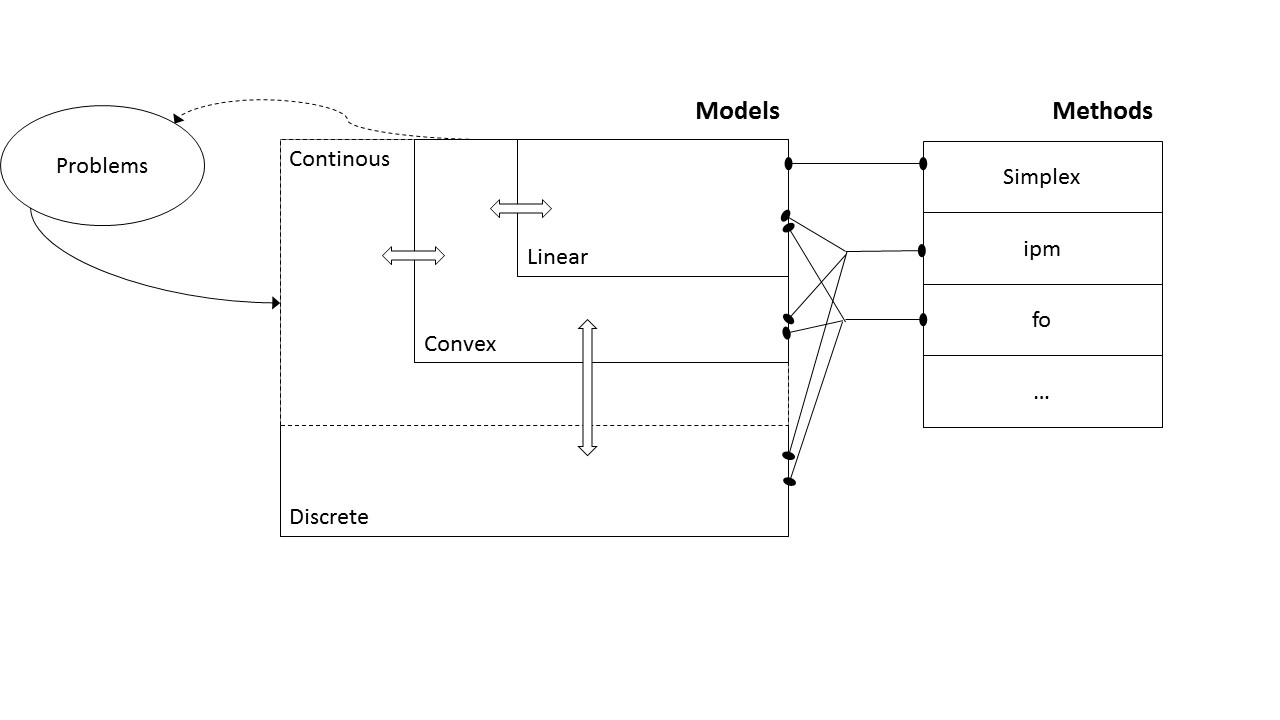
\includegraphics[width=\textwidth]{./images/Course1_Slide1.JPG}
\caption{Visualization of the relation between models and methods}
\label{Figure1}
\end{figure} 

AMPL works by first reading a text file which contains all the useful information of the model, this file usually ends in ".mod", it then parses it and tries to solve the problem. Parameters, variables, objective function and constraints are all defined in this file. The solving part is done by communicating with a solver, AMPL gives it all the information, the solver then sends back the solution. 
Consider the following optimization problem:

\begin{align*}
          &\min \, c^Tx  \\ 
       	 & Ay\le b\\
	 & l\le y\le u
\end{align*}
\\

For this problem AMPL will give the solver the usefull values ($c$,$A$,$b$,$l$,$u$,...) it neads to solve the problem. There exists quite a few of these solvers, some mode adapted to certain model types (linear, convex,...). 
We have for example:

\begin{itemize}
  \item minos (basic solver for linear and nonlinear problems)
  \item cplex (can be used for linear, convex, mixted integer models)
  \item gurobi (very similar to cplex)
  \item knitro (good for nonlinear models)
  \item $\cdots$
\end{itemize} 

This can be summerized by the next table: 

\begin{tabular}{|C{0.2 \textwidth}|L{0.5 \textwidth}|C{0.2 \textwidth}|}
\hline
Solvers & Problems & Integer variables \\
\hline
\hline
CPLEX, GUROBI & linear optimization and convex quadratic optimization & yes \\
\hline
KNITRO, SNOPT, MINOS & nonlinear optimization & yes for KNITRO but loss of efficiency \\
\hline
BARON & global optimization & no \\
\hline
\end{tabular}

\begin{figure}[h!]
\centering
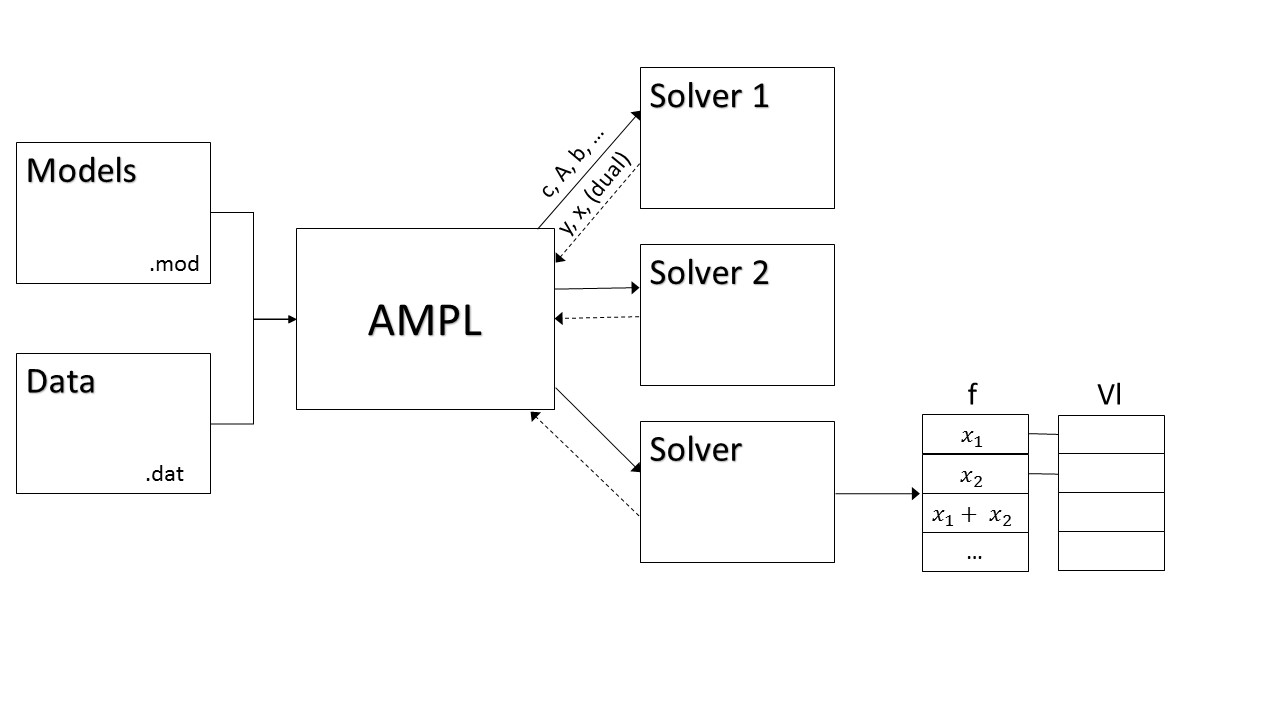
\includegraphics[width=\textwidth]{./images/Course1_Slide2.JPG}
\caption{}
\label{Figure2}
\end{figure} 

AMPL can also work with an additionnal data file (".dat") which is used when parameters are left in the model file. This allows us to avoid changing the entire file when looking at different values of parameters, and only having to change them once in the data file. \\

A few examples and the basic syntax for AMPL can be found in the Tutorials Dropbox, given on Moodle. \\

Everything in AMPL has a name, whether it be variables, constants, or even constraints (which represent a dual variable) and each command and declaration ends with a semicolon (";"). 
Certain commands are worth being reminded here, for example: \\

\begin{itemize}
  \item Changing solvers: \textbf{option solver ... ;}
  \item Displaying dual variable: \textbf{display Protein;}
  \item Displaying variable: \textbf{display Protein.body;}
  \item Reset the whole model: \textbf{reset;}
  \item Chosing a model file: \textbf{data data1.dat;}
  \item Chosing a data file: \textbf{model data1.mod;}
  \item Solving the chosen model: \textbf{solve;}
\end{itemize} 





	
	



% \part{Exercices}



\end{document}
